\documentclass[lettersize,journal]{IEEEtran}
\usepackage{amsmath,amsfonts}
%\usepackage{algorithmic}
\usepackage{algorithm}
\usepackage{array}
\usepackage[caption=false,font=normalsize,labelfont=sf,textfont=sf]{subfig}
\usepackage{textcomp}
\usepackage{stfloats}
\usepackage{url}
\usepackage{verbatim}
\usepackage{graphicx} 
%\usepackage[draft]{graphicx}

\usepackage{cite}
\usepackage{xcolor}
\usepackage{threeparttable}
\usepackage{multirow}

\usepackage{url}
\usepackage{hyperref}

\hyphenation{op-tical net-works semi-conduc-tor IEEE-Xplore}

\usepackage{amssymb}  % assumes amsmath package installed
\usepackage{algorithmicx}
\usepackage{algpseudocode}
\floatname{algorithm}{Algorithm}
\renewcommand{\algorithmicrequire}{\textbf{Input:}}
\renewcommand{\algorithmicensure}{\textbf{Output:}}


\begin{document}

\title{Non-revisiting Uniform Coverage by Edge Subdivision of Arbitrary Meshes}

\author{Tong Yang$^1$~\IEEEmembership{Student Member,~IEEE}, Jaime Valls Miro$^2$~\IEEEmembership{Member,~IEEE}, Yue Wang$^{1*}$ and Rong Xiong$^1$
\thanks{$^1$ Tong Yang, Yue Wang, and Rong Xiong are with the State Key 
Laboratory of Industrial Control and Technology, Zhejiang University, P.R. China.}
\thanks{$^2$ Jaime Valls Miro is with the Robotics Institute at the University of Technology Sydney (UTS:RI), Sydney, Australia.}
\thanks{$^*$ Corresponding author, %\newline \indent
{\tt\small rxiong@zju.edu.cn.}}
}

\maketitle
\begin{abstract}
A novel mechanism to generate a non-revisiting uniform coverage (NUC) path on an arbitrarily shaped object surface is presented in this work. 
Given a non-planar surface, the non-zero curvature makes traditional homeomorphic fitting of regular template coverage paths from planar regions onto the 
object surface non-distance-preserving. 
Any coverage path with a realistic tooling size derived in this way will suffer from overlaps and missing gaps when transformed onto the object surfaces, 
unable to uniformly cover the target.
To overcome this, the NUC problem is modelled as a non-repetitive sequencing of the full set of uniformly distributed points on a mesh surface, 
where the number of points can be proportionally set in accordance with the area affected by the tooling size on the surface. 
After a prior re-meshing of the object surface into a uniform unstructured mesh, a geometric coverage planner is proposed that proves
that the refined polygonal mesh resulting from mesh subdivision whereby all facets edges are split once, must admit a path solution to the NUC problem.
Extensive simulation examples and real-world illustrations are presented to prove the validity of the proposed strategy in realistic settings. 
The proposed scheme is able to achieve 92.45\% coverage on benchmark tests, outperforming comparable coverage 
algorithms, e.g. a homeomorphic Boustrophedon mapping which can at best achieve 72.37\% coverage.
An accompanying video is supplied for added clarity, and an open-source implementation has also been made available. 
\end{abstract}

\begin{IEEEkeywords}
Coverage Path Planning, Uniform Coverage, Mesh Subdivision
\end{IEEEkeywords}

\section{Introduction}
The \textit{Coverage Path Planning} (CPP)~\cite{Galceran2013A} task on a non-planar surface seeks to reveal a path such that the number of 
traversed points on the superficial is maximised. 
The problem is present in a wide range of industrial applications, such as terrain coverage~\cite{Eiben2020Problem}, bathymetric surveying~\cite{Galceran2013Planning}~\cite{Balampanis2017Spiral}, surface inspection~\cite{Ellefsen2017Multiobjective} or agricultural field mapping~\cite{Oksanen2009Coverage}.
In certain situations, uniform surface coverage~\cite{Tam1999Toward}~\cite{Atkar2005Uniform} becomes a critical feature for the resulting path.
This is a special case that takes into consideration the area effected by the tool on the surface, and seeks to maximise the overall surface covered whilst 
minimising the overlap between tool traces. This is apparent for instance in painting tasks~\cite{Chen2008Automated}, contact-based surface inspection~\cite{Liu2020Optimal} 
or marine growth removal from hulls with a water blaster with minimal over-coverage to avoid fatigue cracks~\cite{Hassan2018A}.
This specialised application, referred to as the \textit{Non-revisiting Uniform Coverage} (NUC) task, is the objective of this work. %which are more practical than CPP in industrial applications.

\begin{figure}[t]
\centering
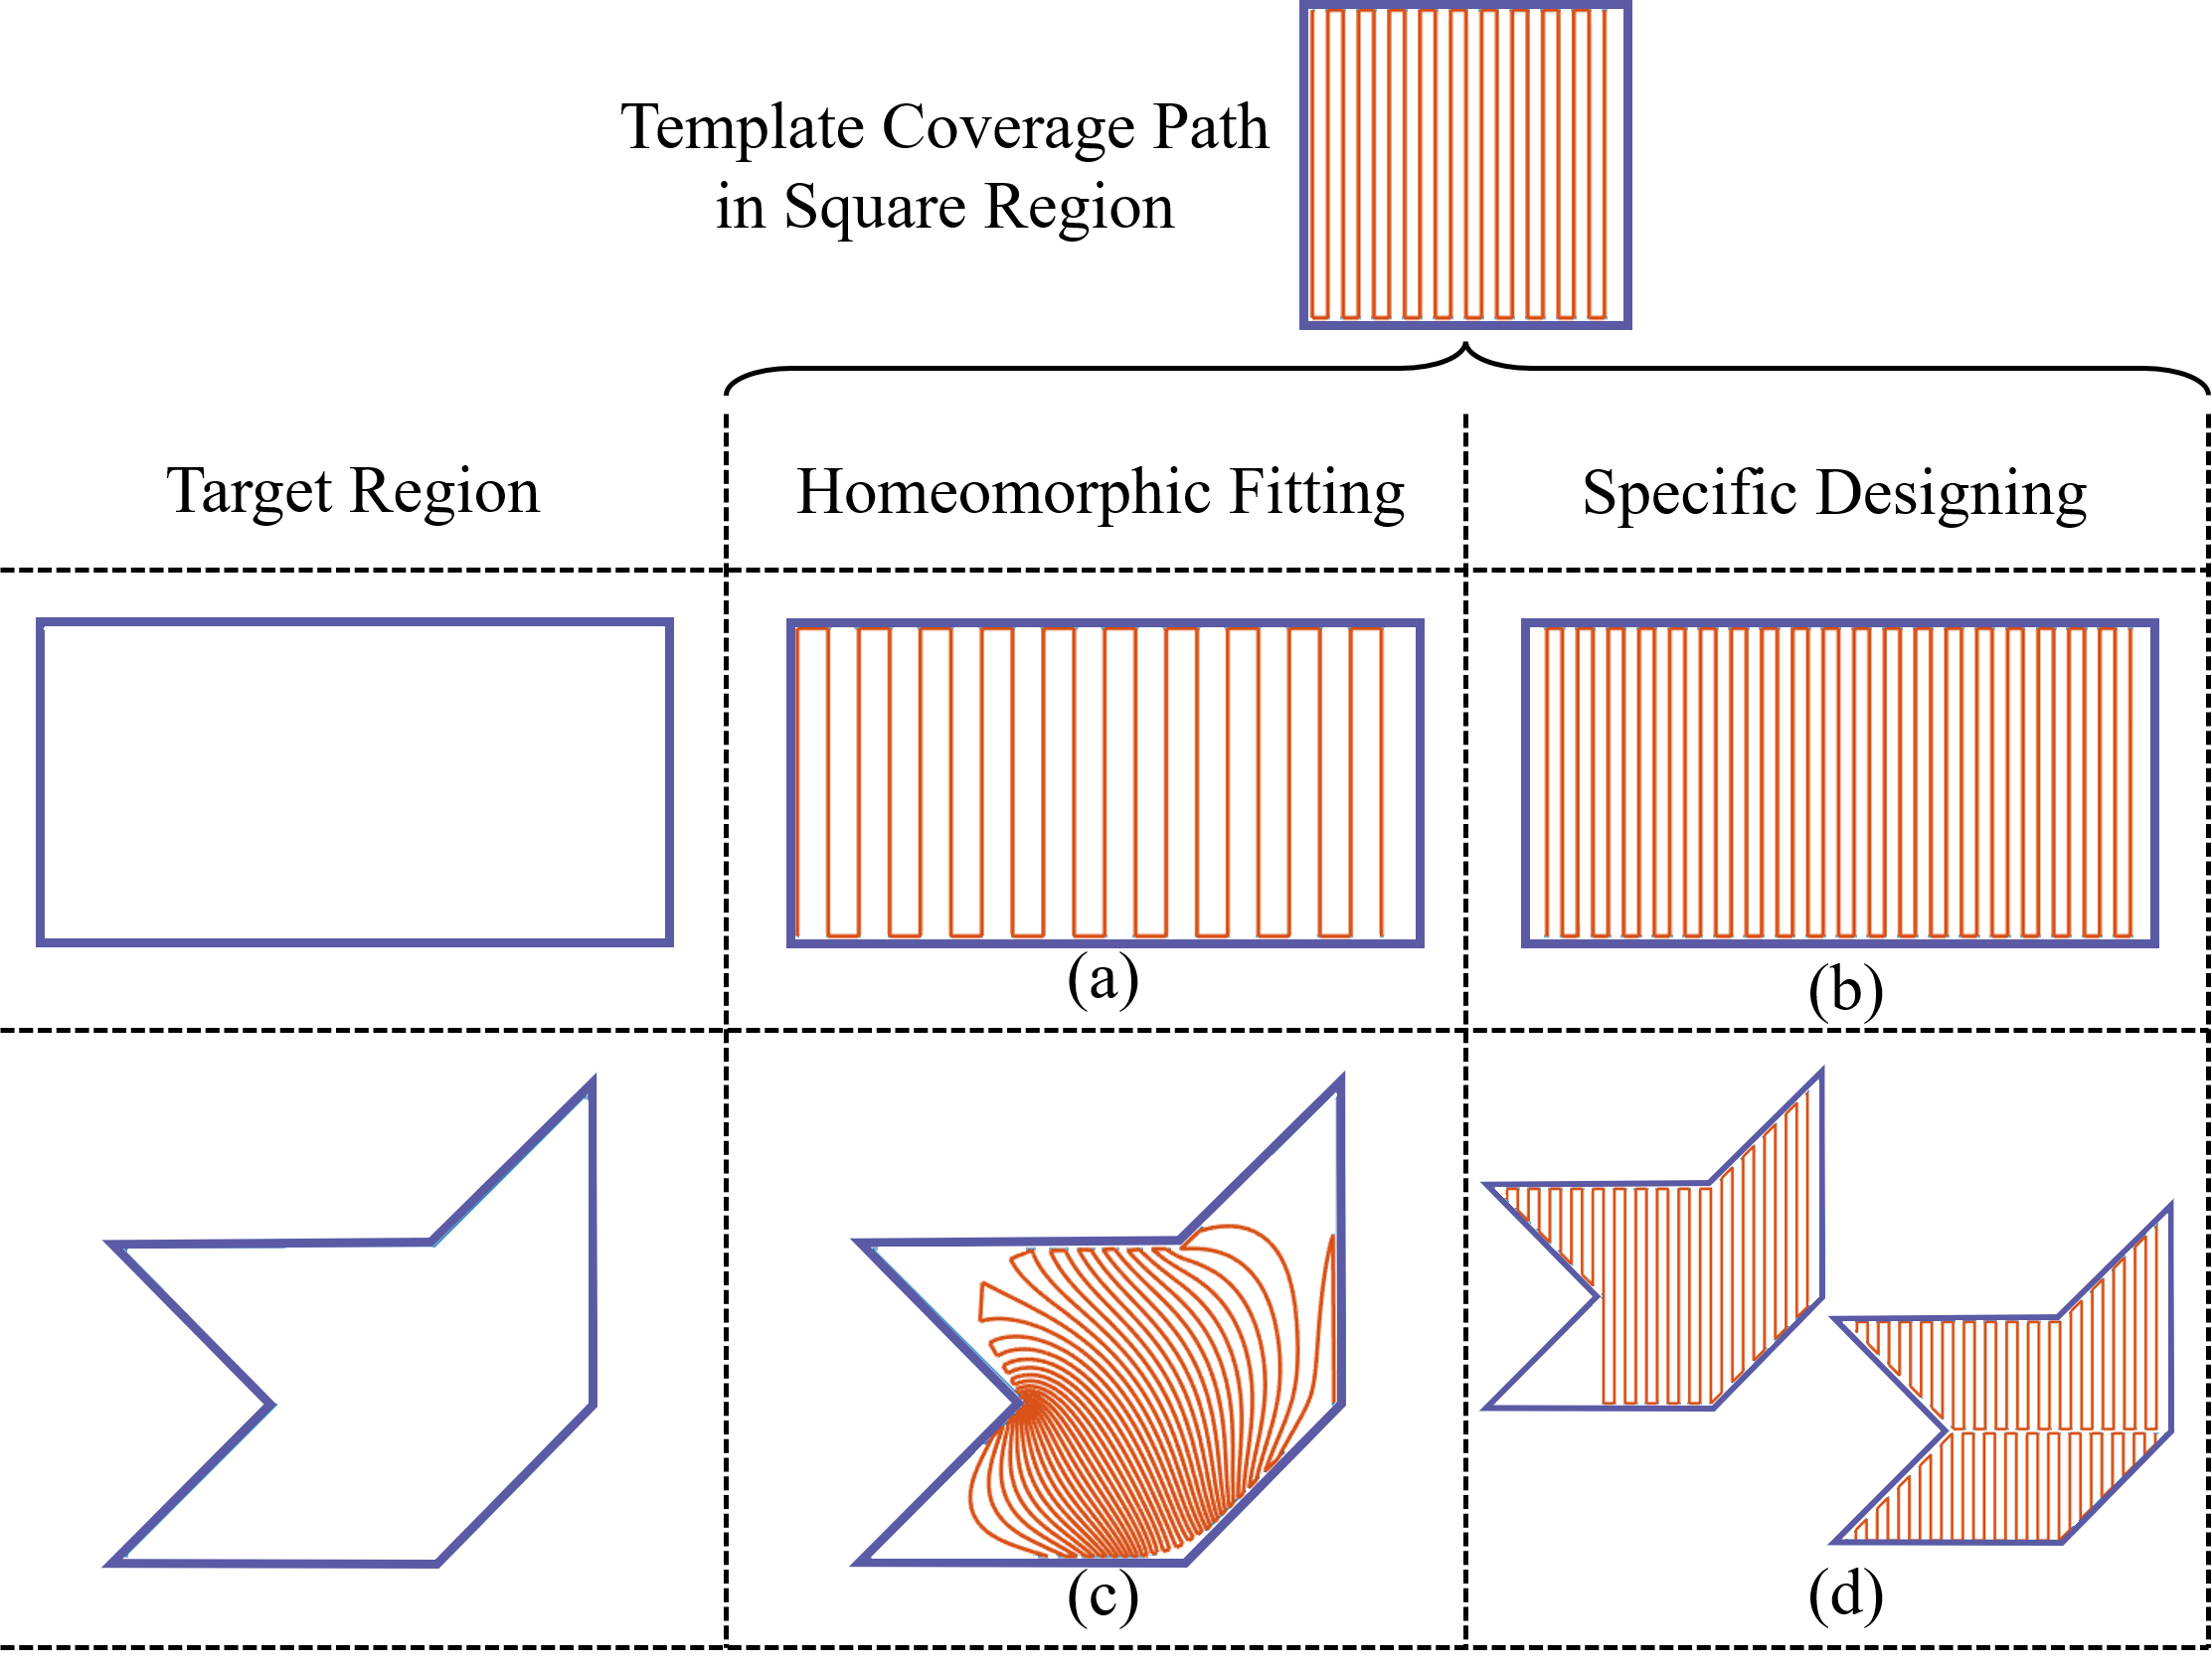
\includegraphics[width=0.44\textwidth]{figures/fig1/fig1_thick}
\caption{Examples of generalising a back-and-forth square template coverage path to two target planar regions, a rectangle (top row) and an arbitrary polygon.
(a) The coverage path generated by homeomorphic fitting cannot uniformly cover the region, with gaps appearing between the path slices as a result of horizontal stretching.  
(b) A specific CPP path design where the number of path turns is calculated in accordance with the length of the rectangle, thus not as established by the template coverage path. 
(c) A conformal area fitting mapping homeomorphism (Schwarz-Christoffel~\cite{Driscoll2002Schwarz}) can be easily fitted into an arbitrary homeomorphic region.
The coverage path is no longer uniform in the target region, leading to overlaps when using a tracing tool, and missing gaps between the path slices. 
(d) Two examples of specific path designs illustrating how for arbitrary regions they do not always exist. In practice, cellular decomposition would be adopted instead, separating the target region into sub-cells and designing a coverage path within each one.
}\label{fig:planar_deformation}
\end{figure}


The CPP for planar regions has been intensively investigated. 
The most popular strategies are based on \textit{cellular decompositions}. 
For polygonal regions, the region is often first decomposed into cells with elemental shapes such as trapezoids, rectangles, and circular regions, and then independently
covered by designing template coverage paths within each cel~\cite{Choset2000Coverage}~\cite{Latombe2012Robot}~\cite{Sadat2015Fractal}~\cite{Hassan2018A}.
For non-polygonal regions, grid-based discretisations~\cite{Gabriely2002Spiral}~\cite{Cabreira2019Grid} are adopted to approximate the coverable region into grids, and template coverage paths~\cite{Choi2009Online} are designed as gridmaps. 
%No optimality or continuity can be derived for this class of solutions. 

An alternative set of algorithms generalise the coverage solution of standard template regions into arbitrary target regions, where the key step is a 
homeomorphic transformation between the two regions. 
Two simple examples of planar homeomorphisms from a unit square to a rectangle and an arbitrary polygonal area are illustrated in Fig.~\ref{fig:planar_deformation}. 
Mathematically, as long as the regions have the same number of ``holes"~\cite{Wu2019Energy} (as in the example), a homeomorphism always exists, whereby the template coverage motion in the unit square 
(e.g., the back-and-forth motion shown in the figure) can always be deformed to fit into the target surface. 
However, solving for the NUC problem is non-trivial because metric distances cannot be preserved by homeomorphic mappings, as illustrated by cases Fig.~\ref{fig:planar_deformation} (a) and Fig.~\ref{fig:planar_deformation} (c). 
More formally, no homeomorphic mapping can simultaneously preserve both the topological layout of a coverage path and the uniformity of the resulting coverage path. 
The problem is further compounded when the surface is non-planar. Due to non-zero curvature at every point on the surface, projecting a template coverage path 
onto a non-planar surface will always render a non-uniform path in the target region. 
An illustrative example projecting various planar coverage solutions onto a saddle grid surface is shown in Fig.~\ref{fig:saddle}. % TONG - I think is a bit unfortunate we don't show the actual planar paths, as per e.g. Fig 6.

Save from simpler objects which can be suitably described by analytical expressions, 3D surfaces are geometrically modelled by polygonal meshes. 
A closer inspection at the NUC problem from a meshing perspective offers insightful observations into the structure of the problem that lends itself to an alternative solver 
proposition that readily reveals uniform coverage paths for non-planar surfaces. 
Coverage routes obtained by homeomorphic fitting as described above can be effectively regarded as a set of ordered waypoints drawn on the structured convex polygon selections 
that make up the polyhedral surfaces, e.g. the grid facet centers in Fig.~\ref{fig:saddle} (left) and (middle).
Whilst paths must be non-uniform as subjected to the unavoidable phenomenon that occurs when projecting a planar coverage path onto a non-planar surface, it is however possible to obtain a set of waypoints that lay \textit{uniformly distributed} on the surface~\cite{Obeidat2009Intelligent} when the mesh is unstructured, as  
shown in Fig.~\ref{fig:saddle} (right) where the center of each facet is covered by a fixed size footprint representing the tool of interest (painting, blasting, polishing, etc.). 
It is clear that with the uniform but unstructured nature of the surface mesh comes the realisation that the waypoints are unordered, and the design of a non-repeated 
visiting sequence of all the waypoints must be solved. Yet the work will prove that by first subdividing all mesh facets, and 
%given the 
%An iterative deformation of an expanding path that relies on 
%the connectedness of the surface facets, and constrained by their adjacency on the mesh, 
by explicitly utilising the local connectivity between adjacent facets on the resulting mesh, a global solution to the NUC path can be obtained by iteratively deforming a path that grows continuously as it incorporates the adjacent facets, until full coverage is achieved. 


\begin{comment}
Looking at the NUC problem from another perspective, the coverage paths obtained by homeomorphic fitting are actually visiting a set of waypoints that are 
under structured selection (e.g., center of grids, Fig.~\ref{fig:saddle:a}).
The paths must be non-uniform because of the non-flatness of the surface. This phenomenon is unavoidable when one projects a planar coverage path onto non-planar surfaces. 
In contrast, it is possible to obtain a set of waypoints that \textit{uniformly distributed} on the surface~\cite{Obeidat2009Intelligent}, for example the center of all facets in Fig.~\ref{fig:saddle:c}, an unstructured mesh. 
However, the waypoints must be unindexed, and the designing of a non-repeated visiting order to waypoints is unsolved. 
\end{comment}

\begin{comment}
% Vastly repeated!!
In this work, a mechanism is proposed to establish non-revisiting uniform coverage on non-planar surfaces. 
The problem is equivalent to non-repetitively covering a set of points that are unordered but uniformly distributed on the target surface. 
This can be further interpreted to covering the center of all facets in an unstructured mesh, and the connectedness of facets is constrained by their adjacency on the mesh. 
The proposed coverage solution departs from decomposing non-planar surfaces into cells, or re-constructing the surface into regular grids for easy adoption of template coverage paths, but explicitly utilising the local connectivity between facets through continuous deformation of paths. 
\end{comment}

The novel contributions in this work can be summarised as: 
\begin{enumerate}
\item Proposing a geometric coverage path planner that constructs a non-revisiting route on a given mesh. 
It only relies on the local connectivity of the mesh facets. As such, it is applicable to all meshes, and it is compatible with any prior high-level cellular decomposition procedure. 
\item Providing proof that whilst not all meshes necessarily admit a NUC solution on their raw facets, a mesh refinement whereby the facet edges are divided once is sufficient to guarantee
the existence of a NUC path in the refined mesh. 
\item Providing proof that no cellular decomposition process is required, hence conferring a fully automated mechanism to the coverage task on any mesh. 
\item Open sourcing an implementation of the proposed solution for use by the wider research community~\footnote{\url{https://github.com/ZJUTongYang/nonrevisiting_uniform_coverage_code}}. 
\end{enumerate}

The remainder of this paper is organised as follows~\footnote{A video complementing the manuscript with details of the work and additional simulations, experimental examples and results can be found at \\\url{https://youtu.be/eb2_LdGoKQA}}. 
Section~\ref{section_related_works} reviews existing literature. 
Section~\ref{section_problem_statement} formally describes the non-revisiting uniform coverage problem and our motivation to the proposed solution methodology. 
Section~\ref{section_algorithm} describes the proposed algorithm to generate a guaranteed coverage path for any non-planar surface by mesh subdivisions and iterative path deformation. 
Experimental results from simulation and by a real NUC path tracking with a robotic manipulator on an actual object are collected in Section~\ref{section_experiment}, with final concluding remarks gathered in Section~\ref{section_conclusion}. 

\begin{figure}[t]
\centering
%\subfloat[]{
%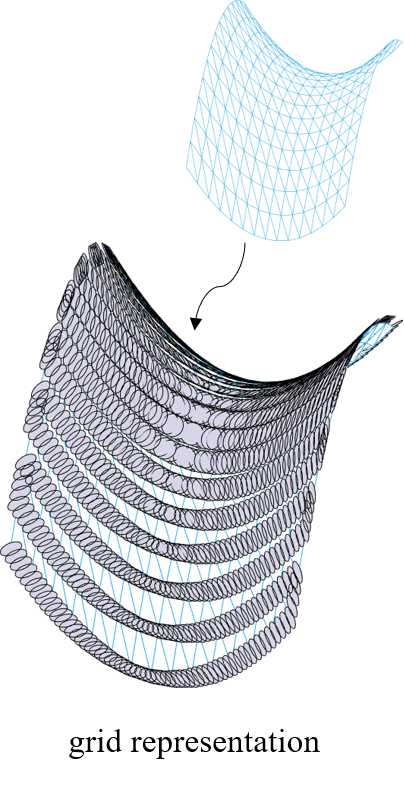
\includegraphics[width=0.15\textwidth]{figures/fig2/saddle_boust_comb}\label{fig:saddle:a}
%}
%\subfloat[]{
%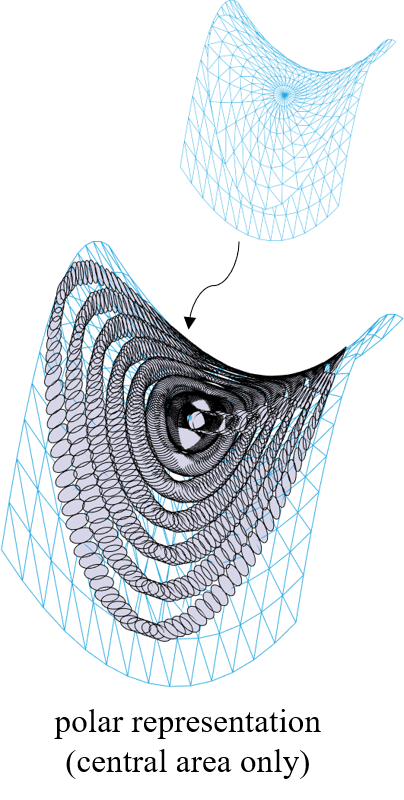
\includegraphics[width=0.15\textwidth]{figures/fig2/saddle_spiral_comb}\label{fig:saddle:b}
%}
%\subfloat[]{
%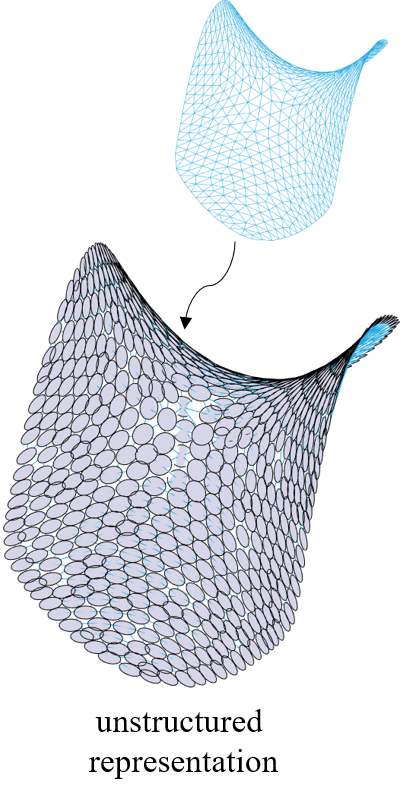
\includegraphics[width=0.15\textwidth]{figures/fig2/saddle_unstructured_comb}\label{fig:saddle:c}
%}
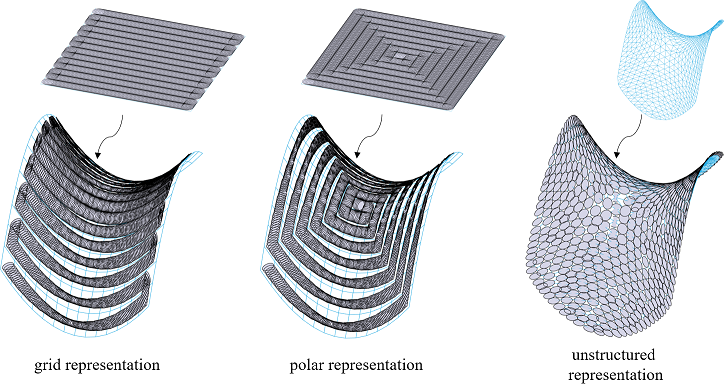
\includegraphics[width=0.44\textwidth]{figures/new_fig2/fig2_smaller}
\caption{
Illustration of the performance of different CPP on a saddle surface. 
The footprint of the tool is visualised in circles in the tangent plane at contact points. 
Boustrophedon path solution (left), spiral motion solution (middle), and a set of CPP waypoints that constitute uniform coverage (right) are depicted here. 
The key step for uniform coverage of an arbitrary non-planar surface is to assume the unstructuredness of waypoints to be non-repetitively visited, where however the designing of a non-revisiting path connecting all such waypoints is non-trivial. 
}\label{fig:saddle}
\end{figure}



\section{Related Works}\label{section_related_works}
There has been a large body of works focused on the coverage task in planar regions~\cite{Wong2003Topological}, where the mainstream approach is a two-stage process: first dividing the target region into several easy sub-regions, the so-called \textit{cellular decomposition}~\cite{Acar2002Morse}~\cite{Ramesh2021Optimal}, and then construct the coverage paths within each sub-region, referred to as \textit{geometric coverage path planning}. 
Generally, cellular decomposition methods~\cite{Mannadiar2010Optimal}~\cite{Brown2016Constriction} have significantly decreased the difficulty of geometric CPP generation, hence the geometric coverage path in sub-regions can be trivially designed~\cite{Bormann2018Indoor}. 
For example, in trapezoidal sub-regions~\cite{Latombe2012Robot} and rectangular sub-regions~\cite{Gabriely2002Spiral} the adoption of boustrophedon paths~\cite{Choset2000Coverage} would be natural, and in circular cells the spiral coverage is straightforward. 
For a non-analytical representation of a region, discretising the coverable region into planar grids~\cite{Gabriely2002Spiral}~\cite{Gonzalez2005Bsa}~\cite{Vselek2018Mobile} has been a popular strategy, since grids can be re-merged into rectangular sub-regions and the problem is eventually solved by one of the aforementioned approaches. 

Coverage solutions of  \textit{non-planar} surfaces are far less mature~\cite{Chen2009Review}~\cite{Huo2021Robotic}. 
Approximating the surface by curvilinear coordinates,~\cite{Tam1999Toward} proposed an extended scanning curve algorithm. It initially constructed a non-uniform back-and-forth path, and then dynamically adjusted the start and termination points of scan lines. 
In analogy to algorithms for planar regions, non-planar surfaces are split into easy sub-regions, and a coverage motion is projected from a planar area onto each sub-region. 
This imposes some challenges: on the one hand, finding a ``suitable'' surface division during the cellular decomposition processes is non-trivial and may require manual intervention~\cite{Zhou2016Sweep}. 
On the other hand, each sub-region is still non-planar, so the lack of uniformity challenge prevails. 
Hence, coverage tasks with consideration of non-zero contact tool sizes have mainly been restricted in the literature to near-flat workpieces ~\cite{Bhatt2020Incorporating}. 
%~\cite{Li2017Interference}. 
%Reducing inspection time for the collision-free coverage of an impeller using a stylus was discussed in~\cite{Wan2019Inspection}. 
In all these approaches, the planar coverage motion was projected onto the target surface, and the inevitable variations in the tool gap width and 
overlapping derived from the tool motion was neglected. 

There is a final family of solutions that do not rely on coverage path patterns, and instead seek uniform coverage curves analytically. 
Isoparametric line sampling for inspection planning was proposed in~\cite{Elkott2005Isoparametric}. 
In considering each facet on the mesh as an analytic planar region, exact geodesic distances of every point to a given source point can be calculated facet-wise~\cite{Liu2010Construction}. 
Then a set of analytical iso-contour curves can be constructed on the given mesh~\cite{Wu2019Energy}. 
Calculating such iso-contour coverage paths is theoretical sound but also costly. Moreover, the detailing in the discrete mesh representation of an object goes beyond 
an analytic approximation of the object surface, meaning that any local change on the mesh vertices' location can thoroughly change the distance fields over the whole mesh.
In practice, the results are similar to an analytic (e.g. polynomial) approximation of the surface, with severe limitations when it comes to being effectively adapted to real-world industrial applications with complex objects to manipulate. 

\section{Problem Modelling}\label{section_problem_statement}
In this section, we firstly state the problem of generating NUC paths on a discrete mesh. 
Then, we provide an analysis of the suggested path deformation process on a discrete mesh, inspiring a sufficient condition that 
guarantees the existence of non-revisiting coverage paths. 

\subsection{Problem Statement}
\textbf{Non-revisiting Uniform Coverage. }
Given a surface $S$ to be manipulated, with surface area ${\rm Area}(S)$, and a tool contact radius defined by $r$, the non-revisiting uniform coverage (NUC) task is defined as finding a non-selfcrossing tool path that will visit all the points uniformly distributed on the surface, whose number is thus defined by ${\rm Area}(S)/(\pi r^2)$. 

Utilising the existing sampling/remeshing algorithms, each sampling point can be regarded as the center of a facet, and a mesh is then well-defined based on the facet adjacencies. Thus the NUC task can be equivalently interpreted in discrete form as: 

\textbf{Non-revisiting Uniform Coverage (discrete). }
Given a surface (or a raw mesh) $S$, it is firstly (re-)meshed into a mesh whose facets are uniformly distributed. 
Denote the mesh as $M = (\{F_i\}, \{V_i\})$, where $\{F_i\}$ is the set of all facets on the mesh, and $\{V_i\}$ is the set of vertices. 
The edge in the mesh is the common boundary of two facets. 
All facets and vertices have been ordered and can be randomly accessed. 
Facets need not have the same number of edges, so unstructured meshes with uniform facet size are particularly applicable. 
A non-revisiting uniform coverage path is a sequencing order of facets, such that
\begin{enumerate}
\item (Connectivity) Each pair of consecutive facets share a common edge. 
\item (Full coverage) All facets are listed in the sequence.
\item (Non-revisiting) Each facet only appears in the sequence for one time. 
\end{enumerate}
A noticeable difficulty in tackling this problem is that, a NUC path does not always exist on arbitrary mesh (see a counterexample in Fig.~\ref{fig:nonexistence}). 
So one has to make some necessary modifications before proposing a generic NUC solution applicable on arbitrary meshes, where for our case is the edge-subdivision process, to be presented in detail in Section~\ref{section_subdivision}. 


\subsection{Motivation}
Our idea originates from the continuous deformation of coverage paths. See Fig.~\ref{fig:continuous_deformation} for a visual illustration. 
Any non-revisiting coverage path is always non-selfcrossing, thus by continuously deforming(shrinking) the coverage path can always be transformed to the locally shortest path connecting the starting facet and the ending facet. 
We are inspired to consider its opposite: Given a trivial initial path, by continuously deforming(stretching) it may be finally transformed to a non-revisiting coverage path. 
The motivation works for both analytic surfaces and discrete meshes, where the existence of such resulting paths in analytic surfaces is trivial. 
Hence in this paper we delve into such a strategy on discrete meshes. 


\begin{figure}[t]
\centering
\subfloat[]{

\includegraphics[width=0.08\textwidth]{figures/nonexistence}\label{fig:nonexistence}
}
\subfloat[]{
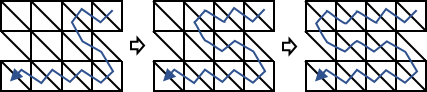
\includegraphics[width=0.36\textwidth]{figures/continuous_deformation}\label{fig:continuous_deformation}
}
\caption{Illustration of non-revisiting coverage paths. 
(a) Case where a non-revisiting uniform coverage path does not exist. 
(b) Illustration of the continuous path deformation process from non-full to full coverage. 
}
\end{figure}

Given a non-full coverage path on the mesh, represented as a sequence $R$ of indices of facets (the bracket $[\cdot]$ means the elements has been in order): 
\begin{equation}
R = [f_1, \cdots, f_m]
\end{equation}
The stretching of path can be represented as replacing a truncated sequence of facets by another longer one, 
\begin{equation}\label{eqn:replace}
\begin{aligned}
\tilde{R} = [f_1, \cdots, f_i, (\tilde{f}_1, \cdots, \tilde{f}_{n}), f_j&, \cdots, f_m]\\
& n > j-i - 1
\end{aligned}
\end{equation}
where the new sequence should still be non-revisiting, 
\begin{equation}
\{\tilde{f}_1, \cdots, \tilde{f}_n\}\cap \{f_1, \cdots, f_i, f_j, \cdots, f_m\} = \varnothing
\end{equation}
Noting that the dropped part $\{f_{i+1}, \cdots, f_{j-1}\}$ will be then unvisited and cause repeated insertions, a practical way may let $j = i+1$ so there is no facet dropped.
The number of covered facets in the coverage path is then non-decreasing and the path will flood the mesh rapidly. 

Analysing in detail to look for sufficient conditions to guarantee the existence of a NUC solution, it is observed that a facet will be inserted into the coverage path if two of its adjacent cells have been consecutively visited. 
This is a sufficient condition for the coverability which points towards a sub-division approach across edges, presented in detail in Section~\ref{section_algorithm}. 


\section{Proposed Algorithm}\label{section_algorithm}
In this section, we present a practical way to subdivide each facet of mesh into a set of sub-facets, such that the resulting refinement of any mesh always ensures the existence of non-revisiting uniform coverage. 
The proof of NUC existence is given by construction, along with the algorithm: 
In each iteration of the proposed algorithm, an unvisited facet will be inserted into the coverage path, whereby the algorithmic complexity of the proposed algorithm is also shown to be linear w.r.t. the number of facets in the mesh. 
The proof of independence to any high-level cellular decomposition is also proven since, thorough this section there is no constraint on the shape of the whole mesh, rectangular or circular, nor simply-connectedness, etc. 


\begin{figure}[t]
\centering
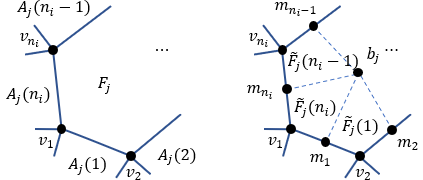
\includegraphics[width=0.36\textwidth]{figures/edge_subdivision}
\caption{Mesh refinement: facet partitioning by edge division. }\label{fig:edge_subdivision}
\end{figure}

\begin{algorithm}[t]
    \caption{Non-revisiting Uniform Coverage}\label{alg:NUC}
    \begin{algorithmic}[1]
        \Require The surface $S$ to be visited, tool size $r$
\Statex \quad($S$ may also be a raw mesh)% A mesh $M = (F, V)$
        \Ensure A sequence of tool waypoints $R$
\State \% Pre-process: Obtaining a uniform unstructured mesh
\State $(\{F_i\}, \{V_i\})$ = UniformRemeshingProcess($S$, $r$)
\State \% Let there be $N$ facets 
\For{$1\leq i \leq N$}
\State $A_i$ = adjacentFacetIndicesInOrder($F_i$)
\EndFor
\For{$1\leq i \leq N$}
\State $\hat{F}_i$ = edgeDivision($F_i$)
\EndFor
\State $\hat{R}$ = $\hat{F}_1$ \% (sequencing order of sub-facets)
\State $Q$ = $A_i$ \% (the queue for unvisited adjacent facets)
\State $C$ = zeros($N, 1$) \% (flags for all covered facets)
\While{$Q$ is not empty}
\State $j$ = $Q(1)$
\State remove $Q(1)$ from $Q$
\If{$C(j)$ == $1$}
\State \textbf{continue}
\EndIf
\State ${\rm loc}$ = $-1$
\For{$i$ in $A_j$}
\If{$C(i)$ == $1$}
\State ${\rm loc}$ = $i$
\State \textbf{break}
\EndIf
\EndFor
\State ${\rm loc1}$ = index of $j$ in $A_i$
\State ${\rm loc2}$ = index of $i$ in $A_j$
\If{$\rm loc1$ == $1$}
\State ${\rm loc'}$ = size of $A_i$
\Else
\State ${\rm loc'}$ = ${\rm loc1} - 1$
\EndIf
\State ${\rm loc}$ = index of $\hat{F}_i({\rm loc'})$ in $\hat{R}$
\State $\hat{R}$ = $[\hat{R}(1), \cdots, \hat{R}({\rm loc}), $
\Statex \qquad\qquad $\hat{F}_j({\rm loc2}), \cdots, \hat{F}_j({\rm end}), $
\Statex \qquad\qquad $\hat{F}_j({\rm 1}), \cdots, \hat{F}_j({\rm loc2}-1), $
\Statex \qquad\qquad $\hat{R}({\rm loc}+1), \cdots, \hat{R}({\rm end})]$
\State $C(j)$ = $1$;
\State insert $A_j$ to $Q$
\EndWhile
\State $R$ = subFacetCenterOf($\hat{R}$)
\State \Return $R$
    \end{algorithmic}  
\end{algorithm}

\subsection{Edge Subdivision}\label{section_subdivision}
See Fig.~\ref{fig:edge_subdivision} for a visual illustration of the edge subdivision process. 
Given any $n$-edge facet $F_j$, denoting its vertices as $v_1, \cdots, v_n$ in cyclic order, the subdivision of $F_j$ is a set of $n$ quadrilaterals, constructed in a specific way:
Denote the barycenter of facet as $b$ and the midpoint of edge connecting $v_i$ and $v_{i+1}$ as $m_i$, the facet is divided by curves that connect $b_j$ and $v_1, \cdots, v_n$, where for convex facets the curves can be straight line segments. 
The $i$-th sub-facet is defined as the quadrilateral: 
\begin{equation}
[b_j, m_i, v_{i+1}, m_{i+1}], i = 1, \cdots, n
\end{equation}
where the indices are in cyclic order, hence $v_{n+1} = v_1$ and $m_{n+1} = m_1$. 
And the bracket $[\cdot]$ means that the quadrilaterals have the same orientation as $F_j$. 
By the subdivision process, each edge of the original mesh is divided into two sub-edges. 

It should be noted that valid edge subdivision processes are not unique. 
We do as above because in most common scenarios, the triangular mesh cases, such subdivision will split an equilateral triangle to three cyclic quadrilaterals with equivalent circumradius. 
Flexible adjustment of the position $b$ in the facet and $\{v_i\}$ on the edges will improve the uniformity of coverage results, which is beyond the scope of this work. 

\subsection{NUC Solution}
Given any surface, we assume that it has been uniformly re-sampled whose intensity is in accordance with the tool size, and been reconstructed to a connected mesh (e.g., in a Voronoi~\cite{choset2000sensor-based} manner), referred to a re-meshing process. 
So the algorithm aims to non-repetitively visit all facets of an arbitrary mesh. 
The proposed algorithm consists of two steps: subdividing all mesh facets, and iteratively deforming a path towards a NUC solution of all sub-facets.
In this subsection, we take two adjacent facets $F_i$ (with $n_i$ edges) and $F_j$ (with $n_j$ edges) as an example. 

\textbf{Step 1: Subdividing the Mesh. }
First, we find the set of adjacent facets of each facet $F_i$, and collect them as $A_i$ in counter-clockwise order. 
Hence the location of $F_j$ in $A_i$ and the location of $F_i$ in $A_j$ are known, denoted as ${\rm loc1}$ and ${\rm loc2}$ respectively. 
Then, we do subdivisions for each facet following the steps shown in Section~\ref{section_subdivision}, which yields the set of sub-facets
\begin{equation}
\begin{aligned}
\hat{F}_i &= \{\hat{F}_i(1), \cdots, \hat{F}_i(n_i)\}\\
\hat{F}_j &= \{\hat{F}_j(1), \cdots, \hat{F}_j(n_j)\}
\end{aligned}
\end{equation}
where the connectivity between $F_i$ and $F_j$ are now replaced by the adjacency of two pairs of sub-facets $\{\hat{F}_i({\rm loc1} - 1), \hat{F}_j({\rm loc2})\}$ and $\{\hat{F}_i({\rm loc1}), \hat{F}_j({\rm loc2}-1)\}$. 
Here all indices were referred cyclicly, as such $\hat{F}_i(0)$ and $\hat{F}_j(0)$ are actually $\hat{F}_i(n_i)$ and $\hat{F}_j(n_j)$, respectively. 

\begin{figure*}[t]
\center
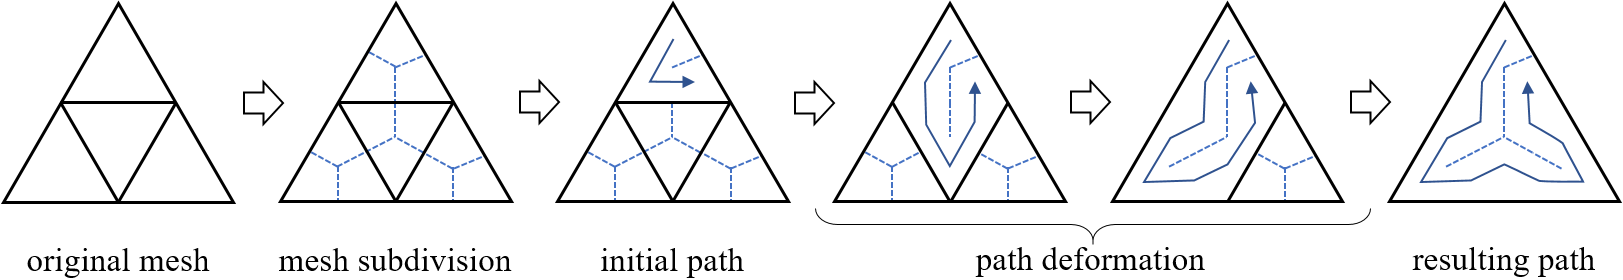
\includegraphics[width=0.8\textwidth]{figures/flowchart}
\caption{Flowchart of the proposed non-revisiting uniform coverage solution by edge subdivision. 
The NUC of the original mesh does not exist. 
However, the NUC of its subdivision always exists and can be obtained by path deformation.  
}\label{fig:flowchart}
\end{figure*}


\begin{figure}[t]
\centering
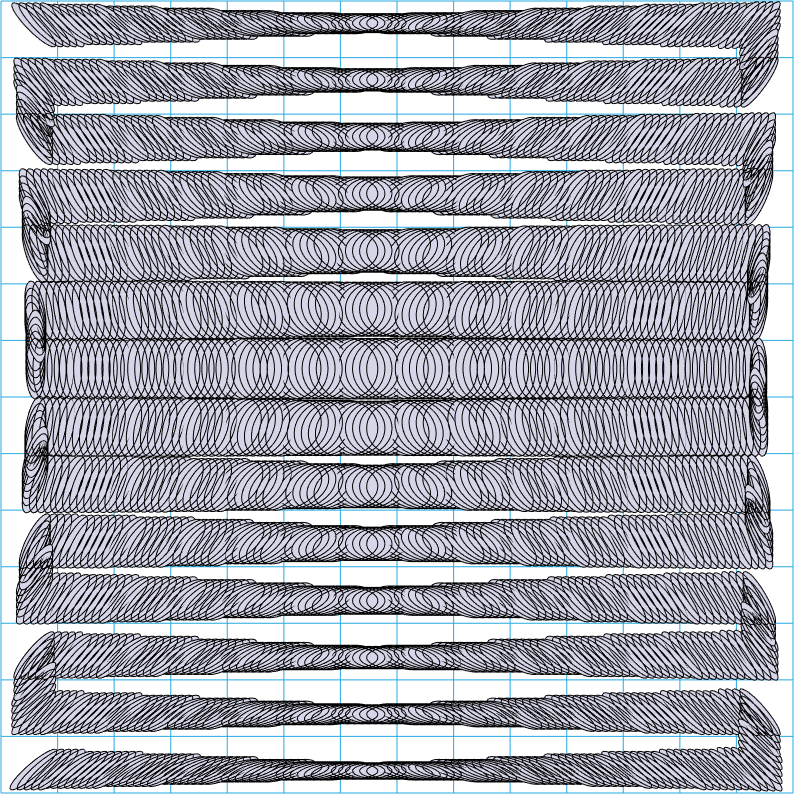
\includegraphics[height=0.14\textwidth]{figures/new_saddle/boust/sparse_top}
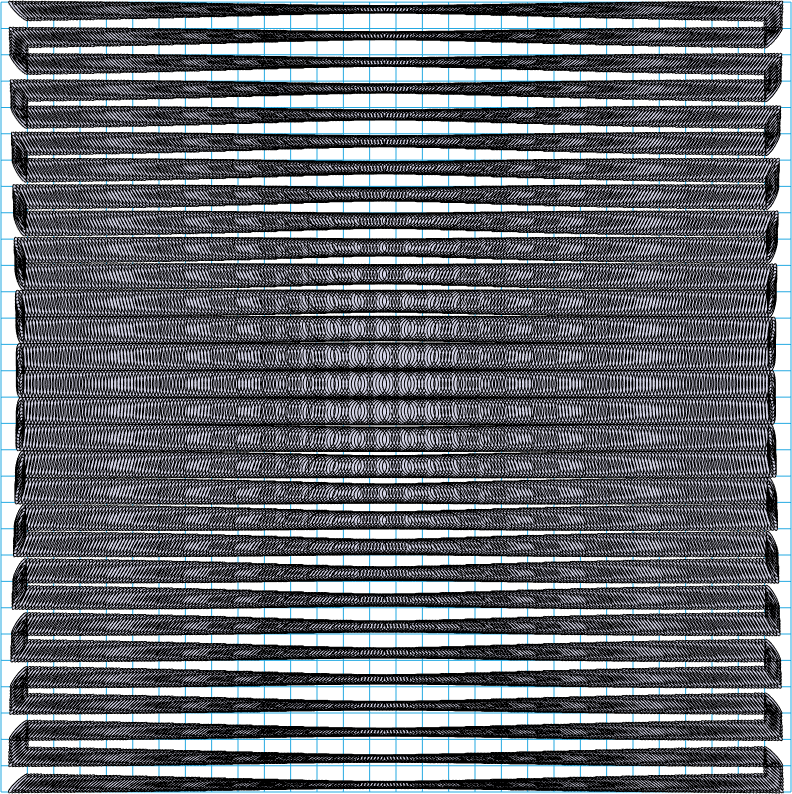
\includegraphics[height=0.14\textwidth]{figures/new_saddle/boust/middle_top}
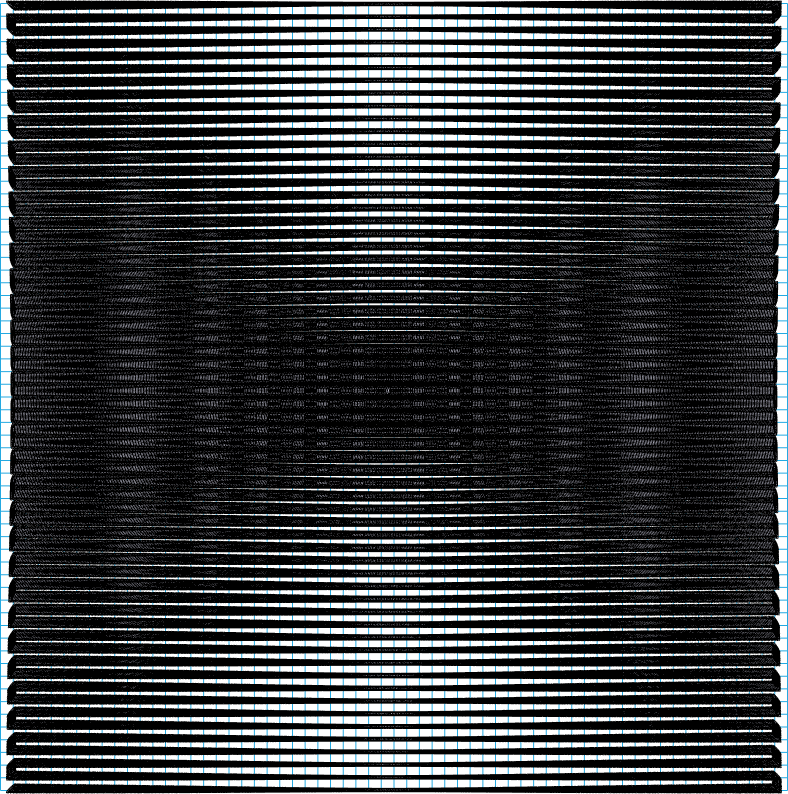
\includegraphics[height=0.14\textwidth]{figures/new_saddle/boust/dense_top}
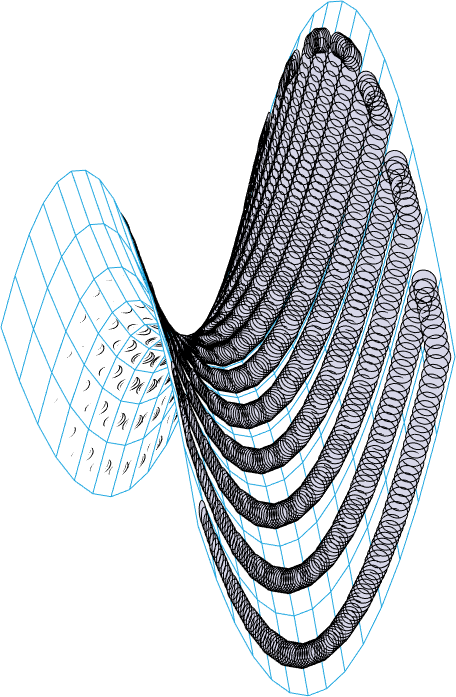
\includegraphics[width=0.14\textwidth]{figures/new_saddle/boust/sparse}
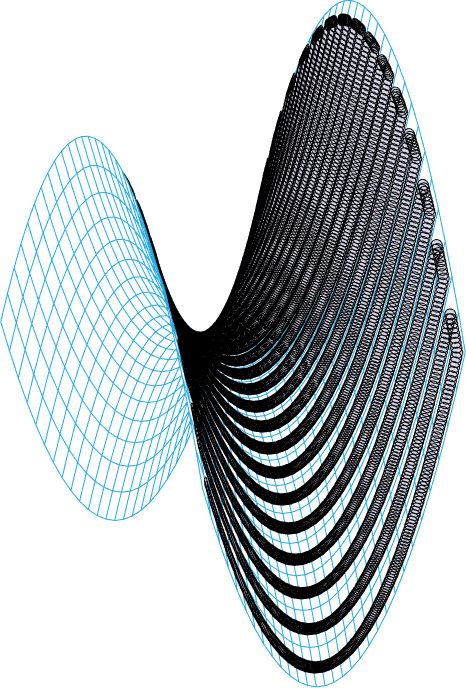
\includegraphics[width=0.14\textwidth]{figures/new_saddle/boust/middle}
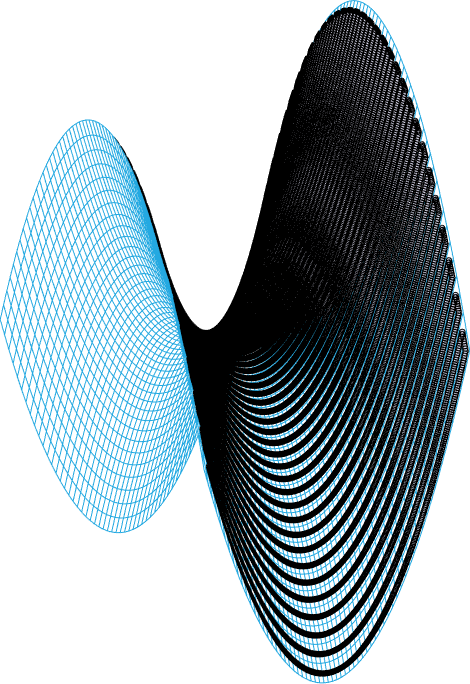
\includegraphics[width=0.14\textwidth]{figures/new_saddle/boust/dense}
%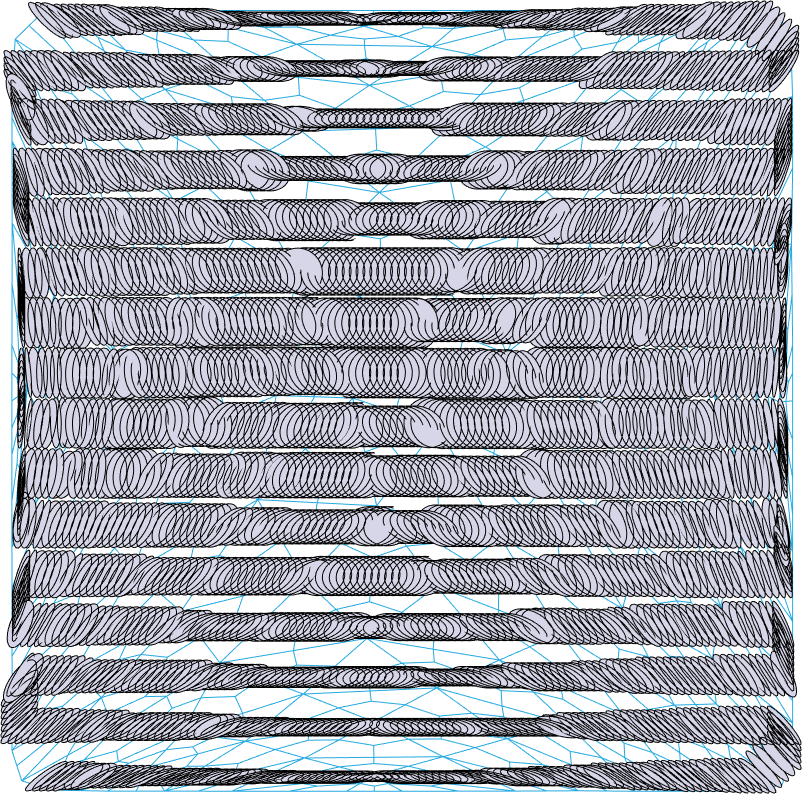
\includegraphics[height=0.14\textwidth]{figures/saddle/boust/006_boust_top_view}
%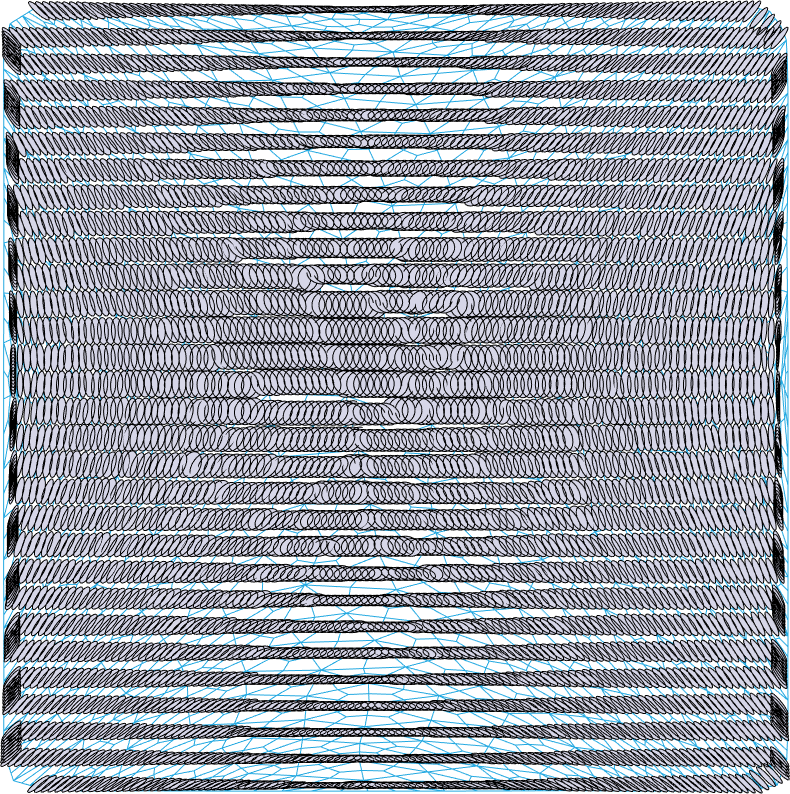
\includegraphics[height=0.14\textwidth]{figures/saddle/boust/003_boust_top_view}
%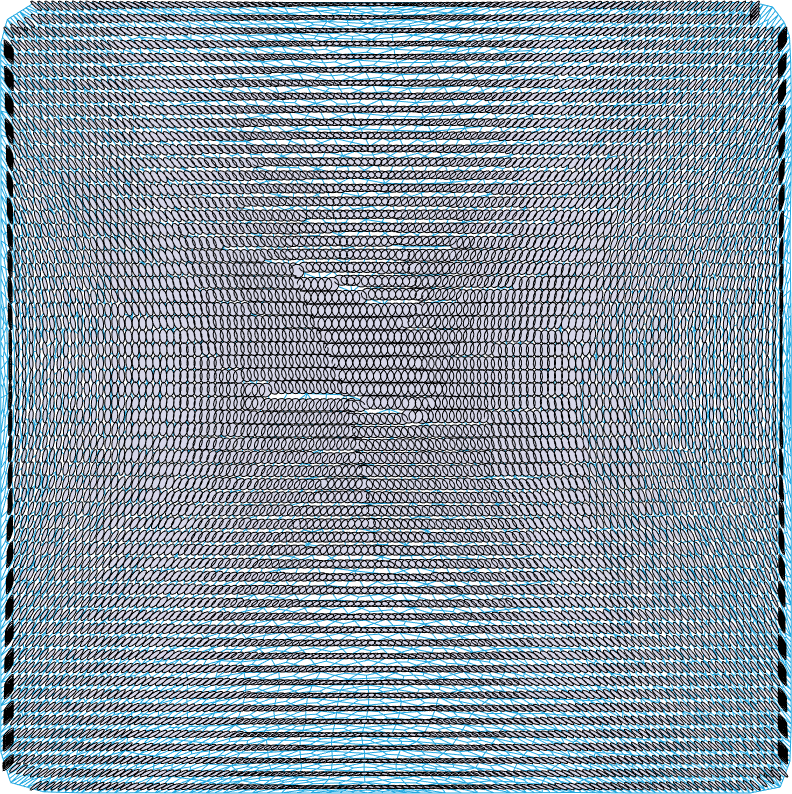
\includegraphics[height=0.14\textwidth]{figures/saddle/boust/0015_boust_top_view}
%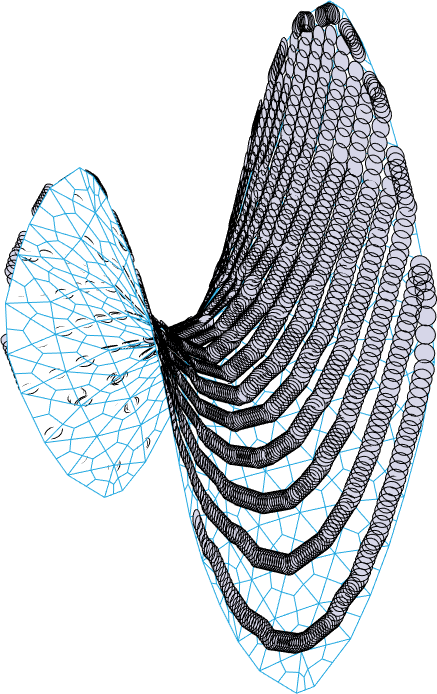
\includegraphics[width=0.14\textwidth]{figures/saddle/boust/006_boust_st_view}
%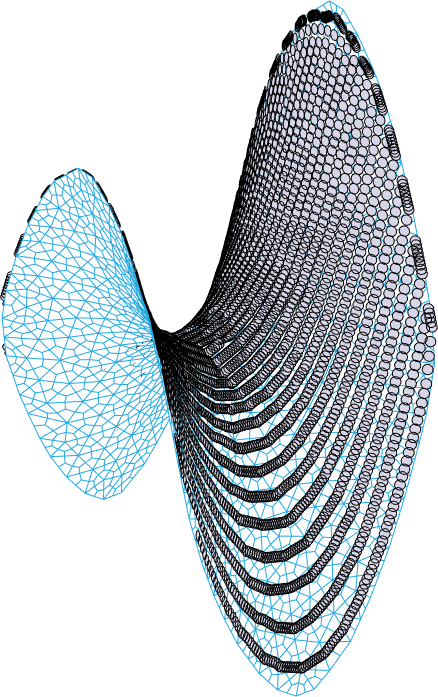
\includegraphics[width=0.14\textwidth]{figures/saddle/boust/003_boust_st_view}
%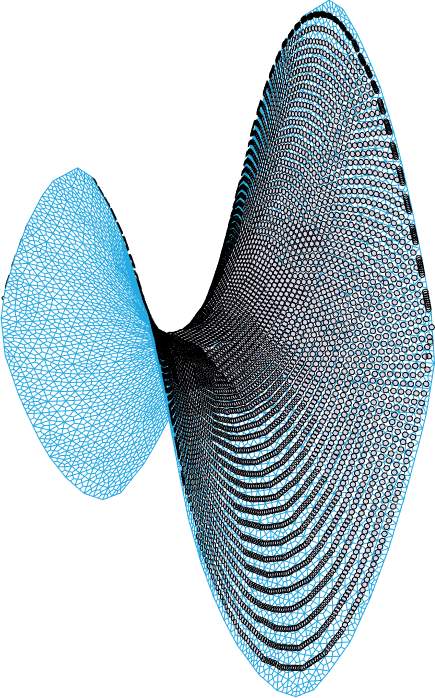
\includegraphics[width=0.14\textwidth]{figures/saddle/boust/0015_boust_st_view}
\caption{
Illustration of horizontal Boustrophedon paths projected vertically onto a sadde surface coverage results (bottom row) with tool size (left) 1.21mm, (middle) 0.57mm, and (right) 0.27mm. 
}\label{fig:exp_boust_horizontal}
\end{figure}


\begin{figure}[t]
\centering
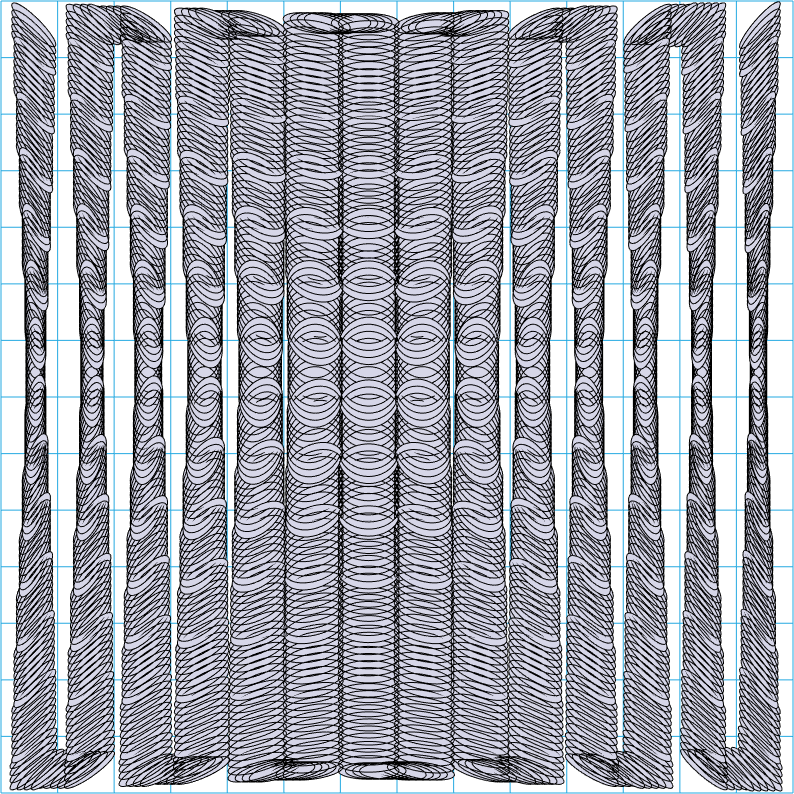
\includegraphics[height=0.14\textwidth]{figures/new_saddle/boust_vertical/sparse_top}
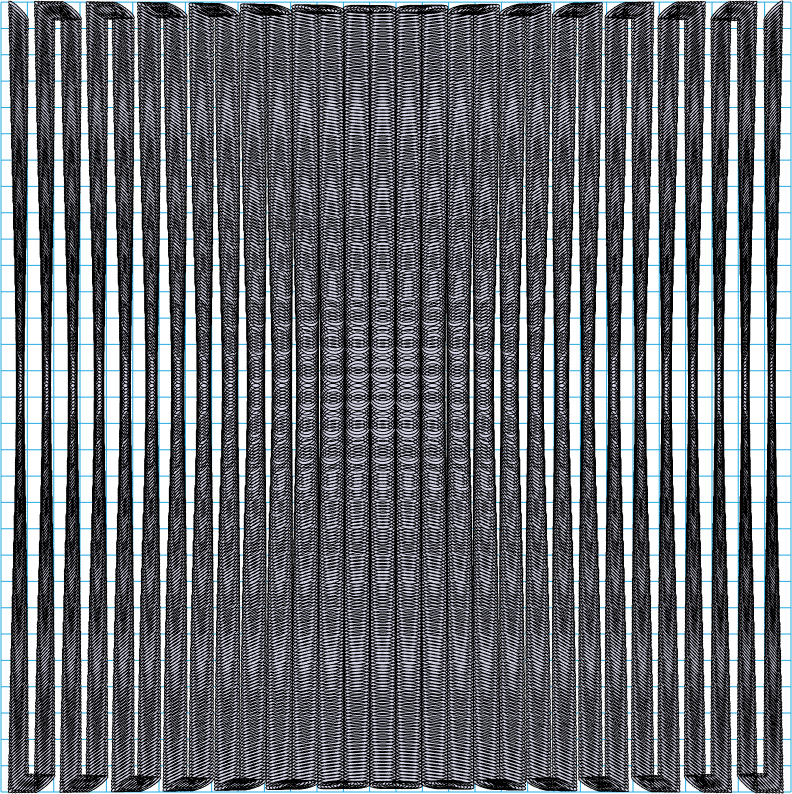
\includegraphics[height=0.14\textwidth]{figures/new_saddle/boust_vertical/middle_top}
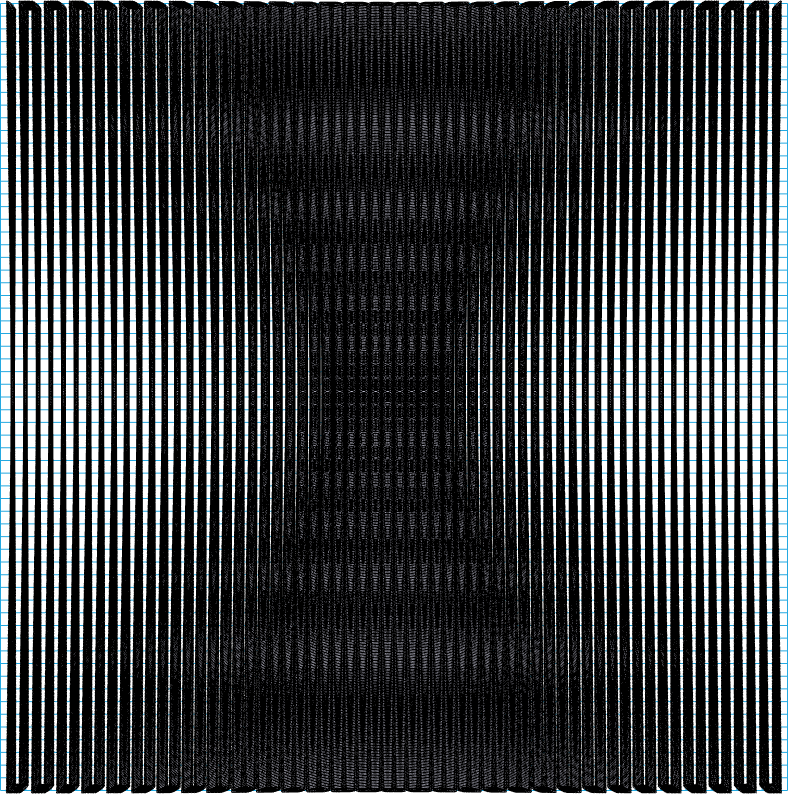
\includegraphics[height=0.14\textwidth]{figures/new_saddle/boust_vertical/dense_top}
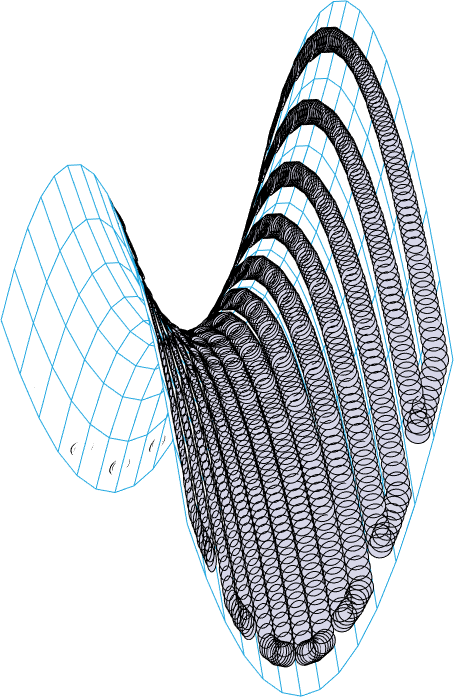
\includegraphics[width=0.14\textwidth]{figures/new_saddle/boust_vertical/sparse}
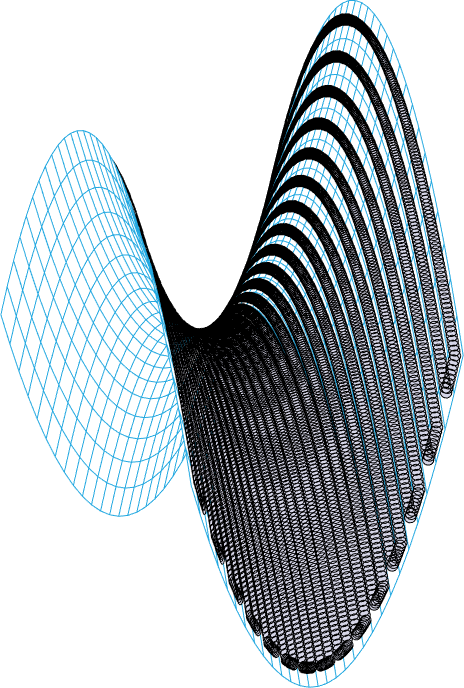
\includegraphics[width=0.14\textwidth]{figures/new_saddle/boust_vertical/middle}
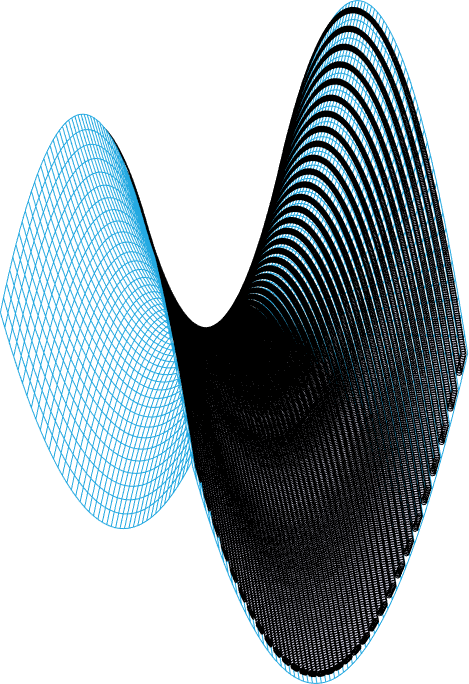
\includegraphics[width=0.14\textwidth]{figures/new_saddle/boust_vertical/dense}
%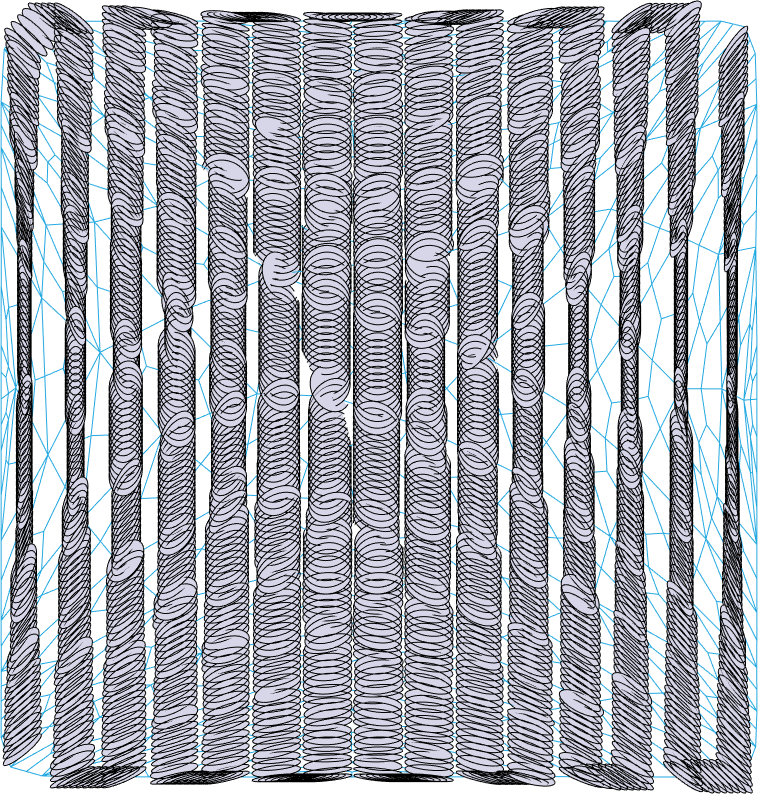
\includegraphics[height=0.14\textwidth]{figures/saddle/boust_vertical/006_boust_top_view}
%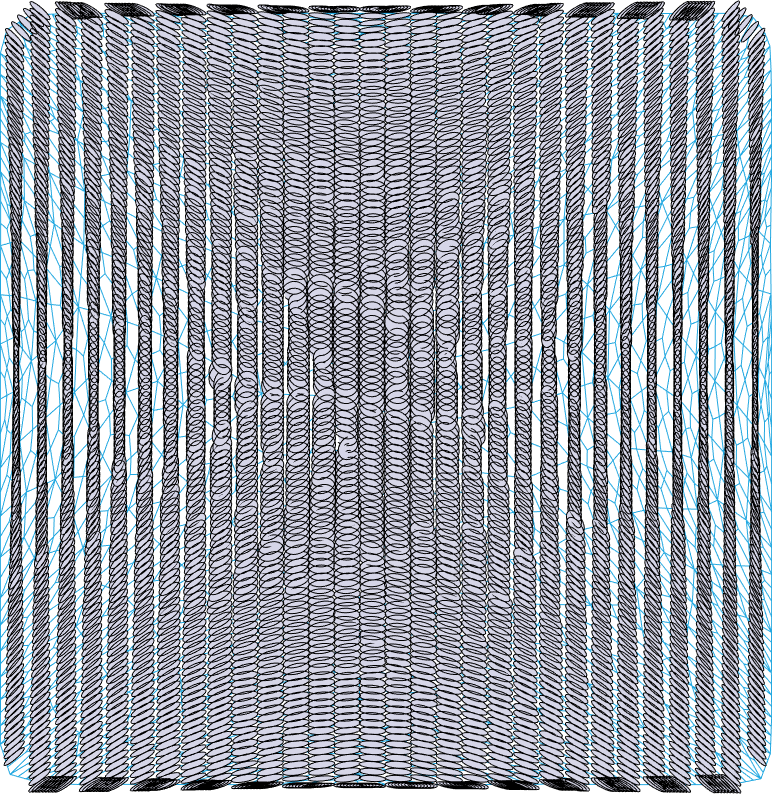
\includegraphics[height=0.14\textwidth]{figures/saddle/boust_vertical/003_boust_top_view}
%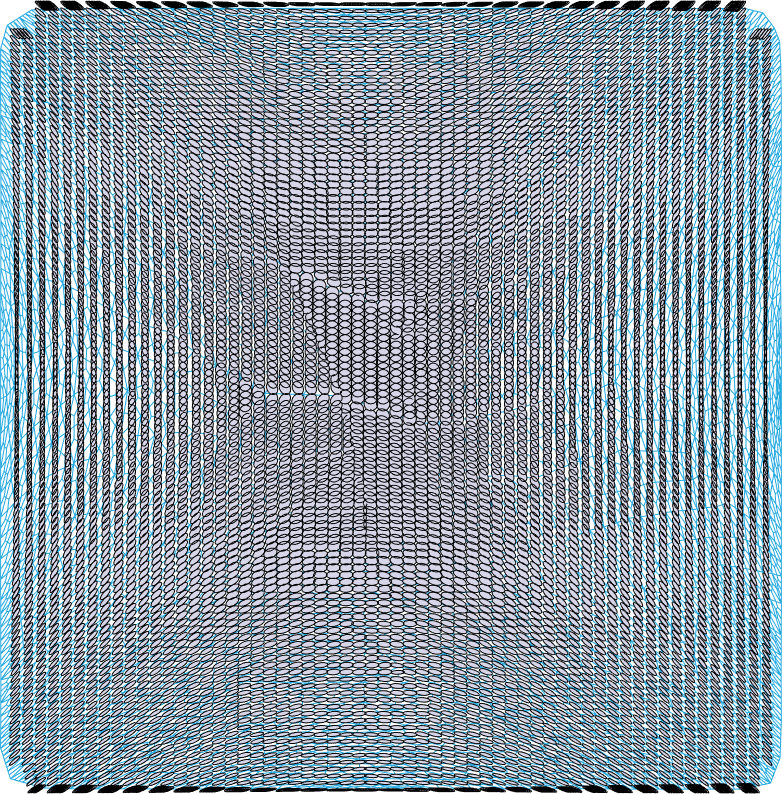
\includegraphics[height=0.14\textwidth]{figures/saddle/boust_vertical/0015_boust_top_view}
%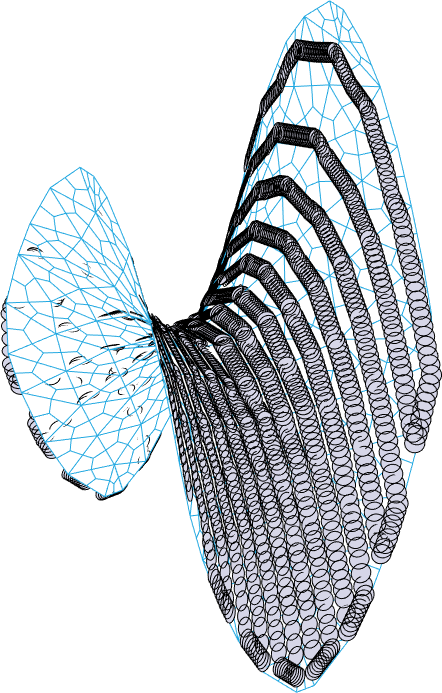
\includegraphics[width=0.14\textwidth]{figures/saddle/boust_vertical/006_boust_st_view}
%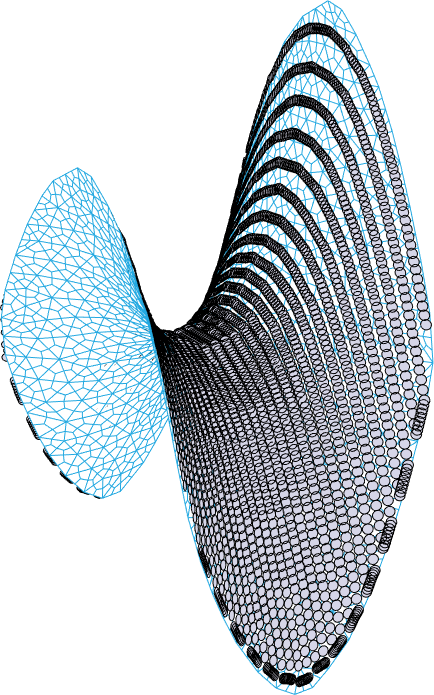
\includegraphics[width=0.14\textwidth]{figures/saddle/boust_vertical/003_boust_st_view}
%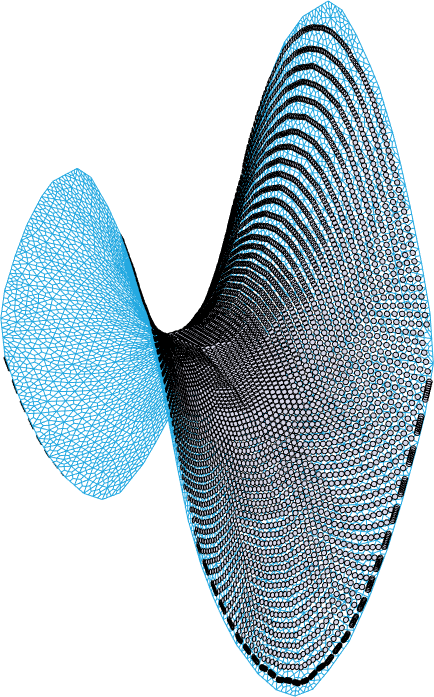
\includegraphics[width=0.14\textwidth]{figures/saddle/boust_vertical/0015_boust_st_view}
\caption{
Illustration of vertical Boustrophedon paths projecting vertically onto the surface with tool size (left) 1.21mm, (middle) 0.57mm, and (right) 0.27mm. 
}\label{fig:exp_boust_vertical}
\end{figure}


\begin{figure}[t]
\centering
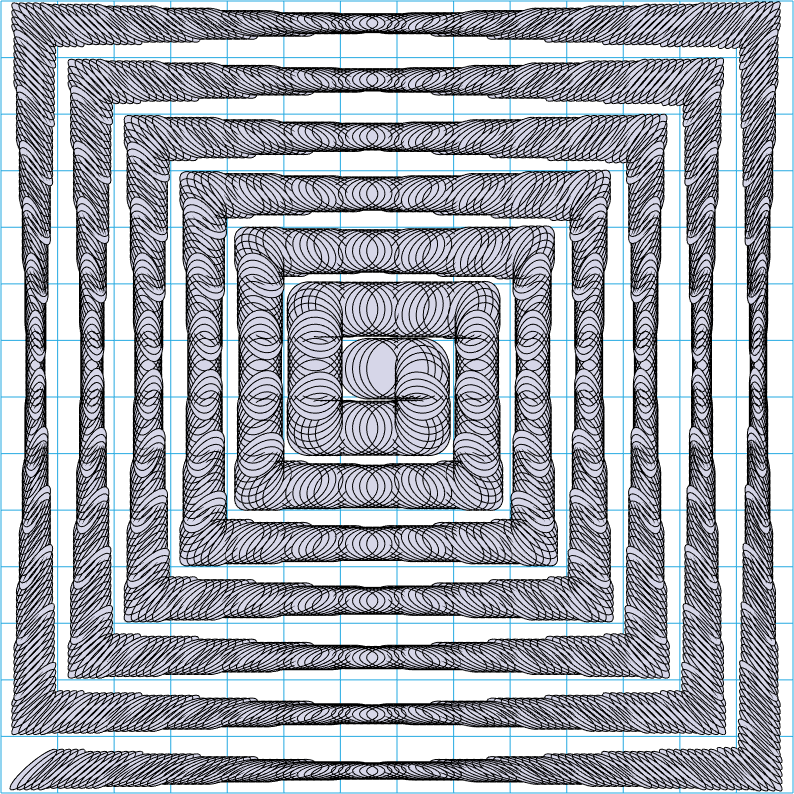
\includegraphics[height=0.14\textwidth]{figures/new_saddle/spiral/sparse_top}
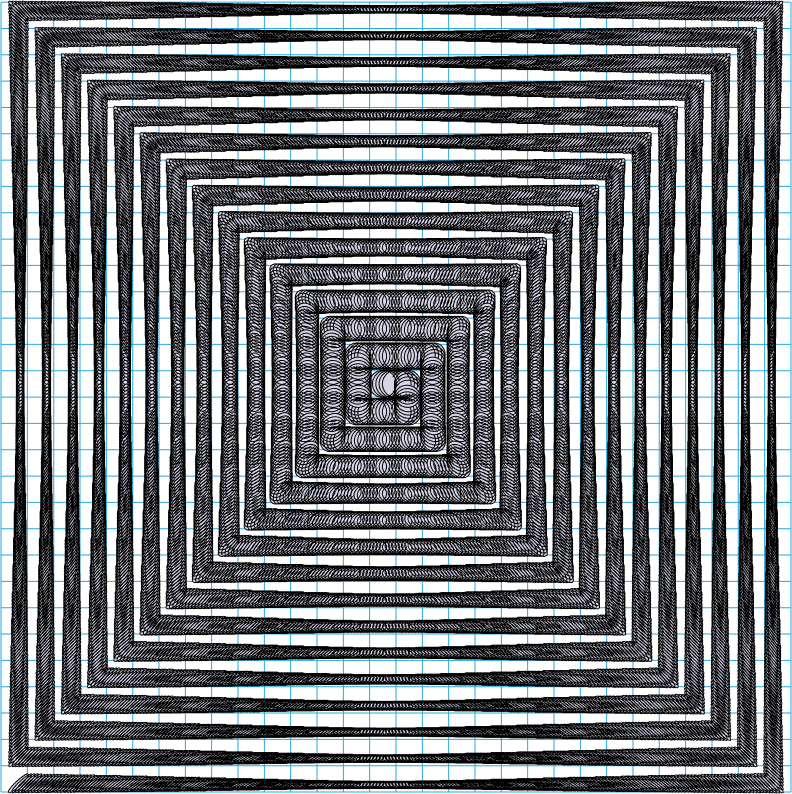
\includegraphics[height=0.14\textwidth]{figures/new_saddle/spiral/middle_top}
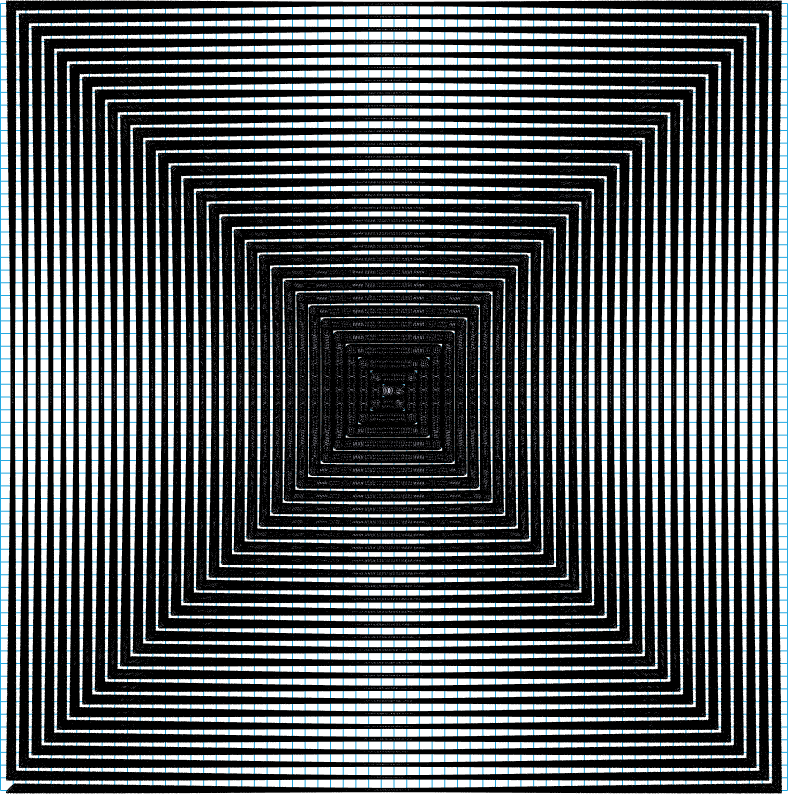
\includegraphics[height=0.14\textwidth]{figures/new_saddle/spiral/dense_top}
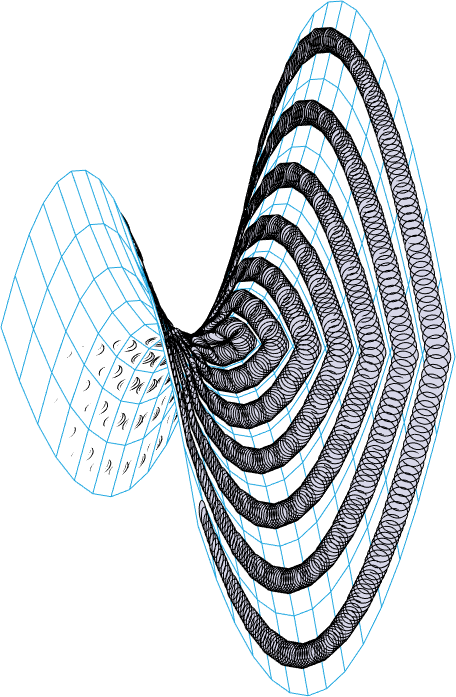
\includegraphics[width=0.14\textwidth]{figures/new_saddle/spiral/sparse}
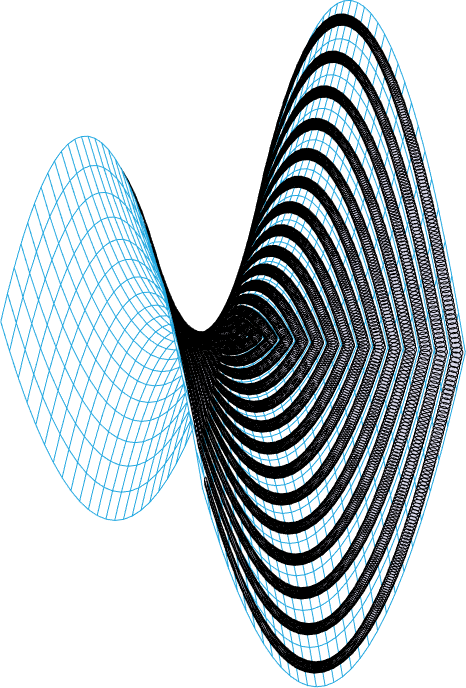
\includegraphics[width=0.14\textwidth]{figures/new_saddle/spiral/middle}
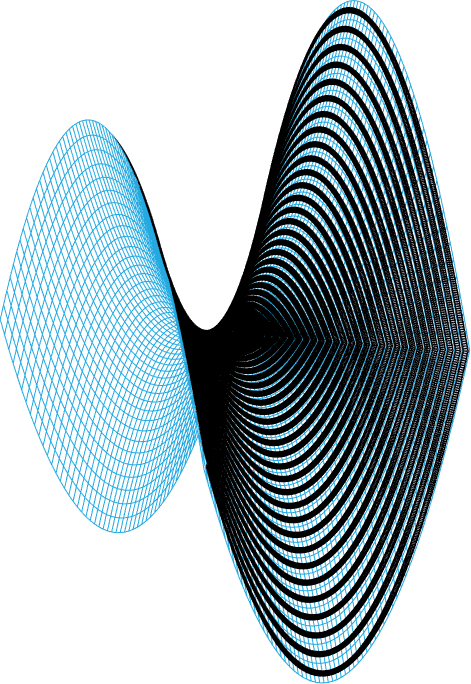
\includegraphics[width=0.14\textwidth]{figures/new_saddle/spiral/dense}
%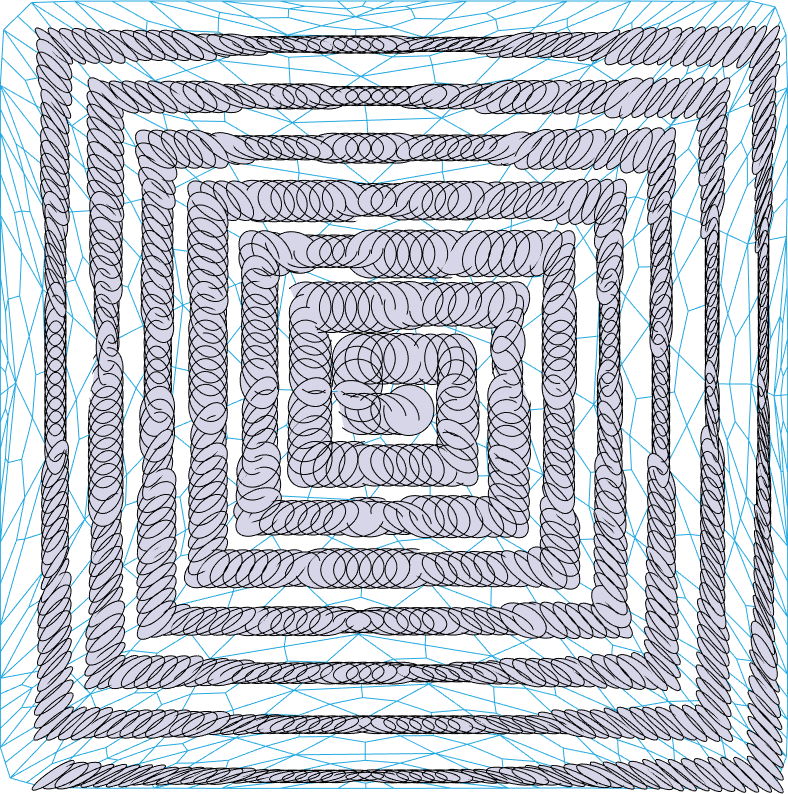
\includegraphics[height=0.14\textwidth]{figures/saddle/spiral/006_spiral_top_view}
%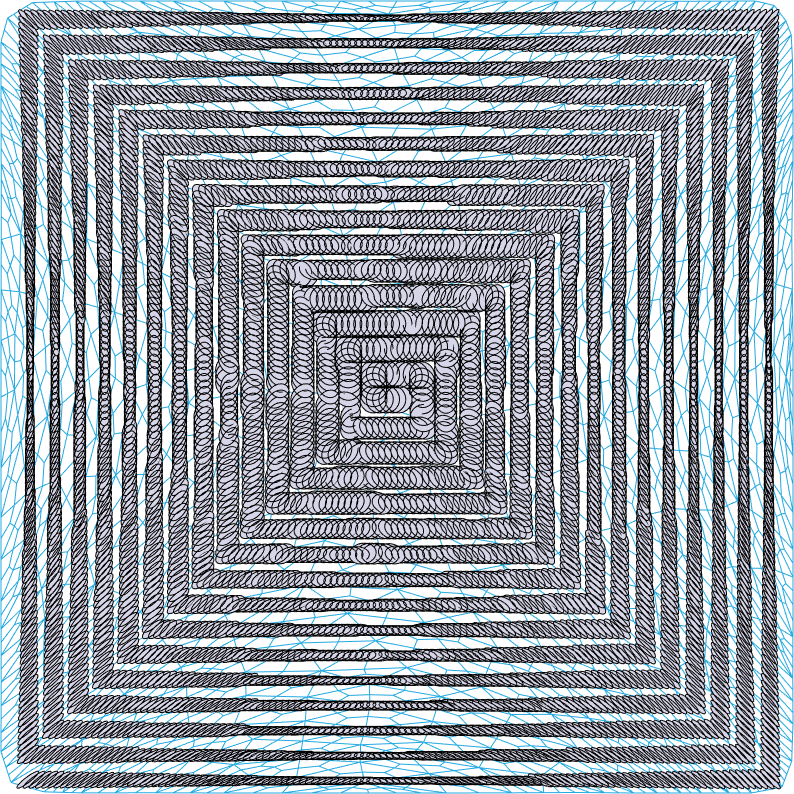
\includegraphics[height=0.14\textwidth]{figures/saddle/spiral/003_spiral_top_view}
%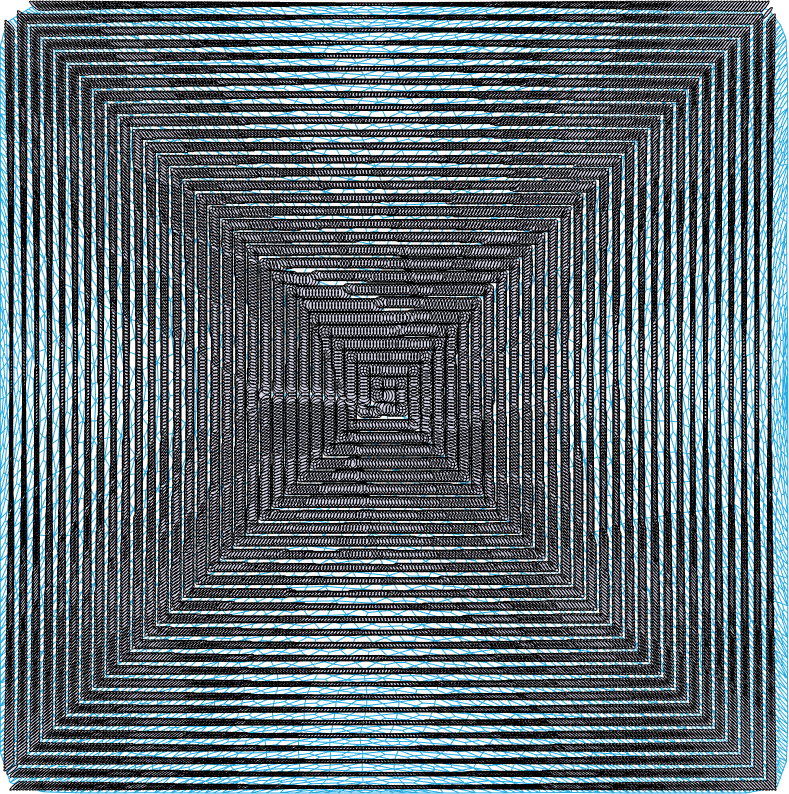
\includegraphics[height=0.14\textwidth]{figures/saddle/spiral/0015_spiral_top_view}
%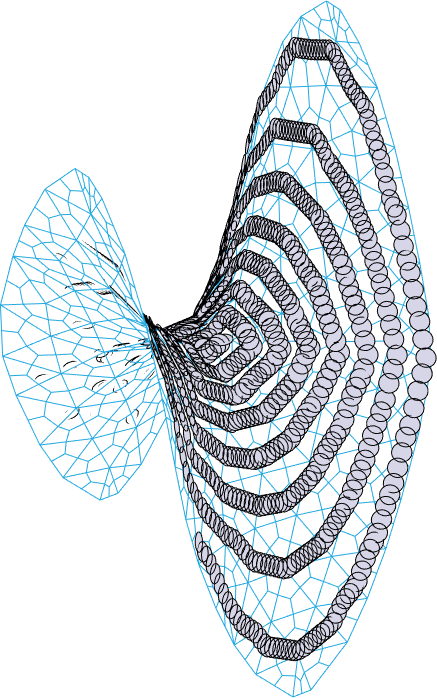
\includegraphics[width=0.14\textwidth]{figures/saddle/spiral/006_spiral_st_view}
%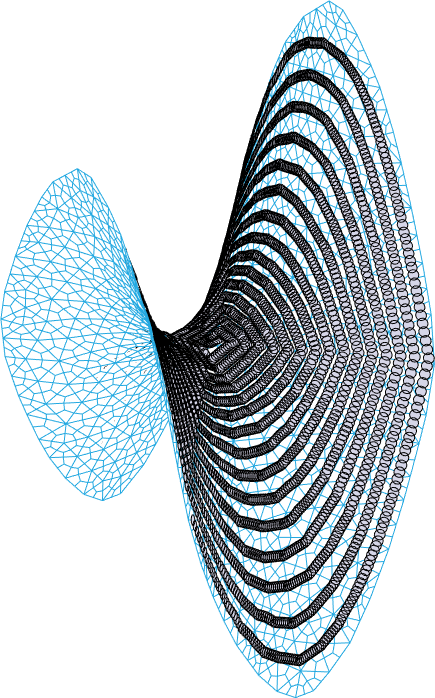
\includegraphics[width=0.14\textwidth]{figures/saddle/spiral/003_spiral_st_view}
%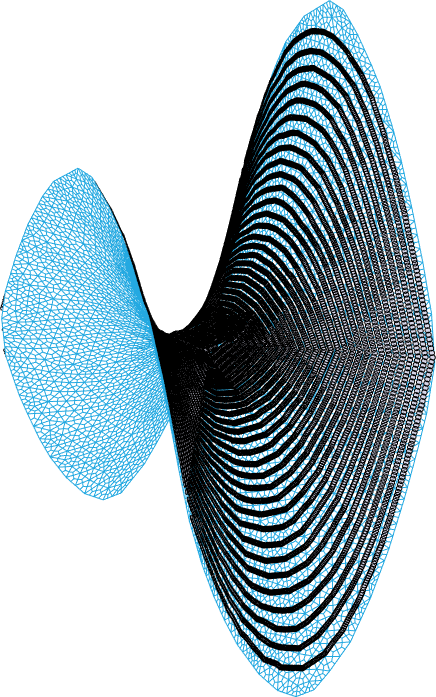
\includegraphics[width=0.14\textwidth]{figures/saddle/spiral/0015_spiral_st_view}
\caption{
Projecting template spiral paths onto the surface with tool size (left) 1.21mm, (middle) 0.57mm, and (right) 0.27mm. 
}\label{fig:exp_spiral}
\end{figure}


\textbf{Step 2: Path Deformation. }
Starting from an initial trivial motion $\hat{R} = \hat{F}_{1}$ (i.e., facet $1$ has been covered), we incrementally incorporate its adjacent facet by continuous path deformation. 
For easy reference of indices, let facet $i$ has been covered and facet $j$ is one of its adjacencies. 
The indices $\rm loc1$ and $\rm loc2$ are defined the same as before. 
We adjust the cyclic order of $\hat{F}_j$ such that it starts from ${\rm loc2}$ and ends at ${\rm loc2 - 1}$, 
\begin{equation}
\begin{aligned}
&[\hat{F}_j(1), \cdots, \hat{F}_j({\rm loc2} - 1), \hat{F}_j({\rm loc2}), \cdots, \hat{F}_j(n_j)]\\
\leadsto & [\hat{F}_j({\rm loc2}), \cdots, \hat{F}_j(n_j), \hat{F}_j(1), \cdots, \hat{F}_j({\rm loc2} - 1)]
\end{aligned}
\end{equation}
and insert it between $\hat{F}_i({\rm loc1}-1)$ and $\hat{F}_i({\rm loc1})$ in $\hat{R}$, 
\begin{equation}
\begin{aligned}
&[\hat{R}(1), \cdots, \hat{F}_i({\rm loc1}-1), \hat{F}_i({\rm loc1}), \cdots, \hat{R}({\rm end})]\\
\leadsto&[\hat{R}(1), \cdots, \hat{F}_i({\rm loc1}-1), \\
&~~\hat{F}_j({\rm loc2}), \cdots, \hat{F}_j({\rm end}), \hat{F}_j(1), \cdots, \hat{F}_j({\rm loc2} - 1), \\
&\qquad\qquad\qquad\qquad\qquad\qquad\hat{F}_i({\rm loc1}), \cdots, \hat{R}({\rm end})]
\end{aligned}
\end{equation} 
Finally, the tool motion is constructed by collecting the centers of sub-facets in $\hat{R}$ in order. 
An algorithmic diagram is presented in \textbf{Algorithm}~\ref{alg:NUC}, and a step-by-step illustration of the construction of the NUC resulting path is shown in Fig.~\ref{fig:flowchart}.  






%\subsection{Remarks}
%\textbf{Algorithmic Complexity. }
%Each facet in the mesh will be only inserted into the coverage path for one time, and no facet is removed from the coverage path. Hence the algorithmic complexity of the proposed algorithm is linear w.r.t. the number of facets in the mesh.





\begin{figure}[t]
\centering
%\subfloat[NUC]{
%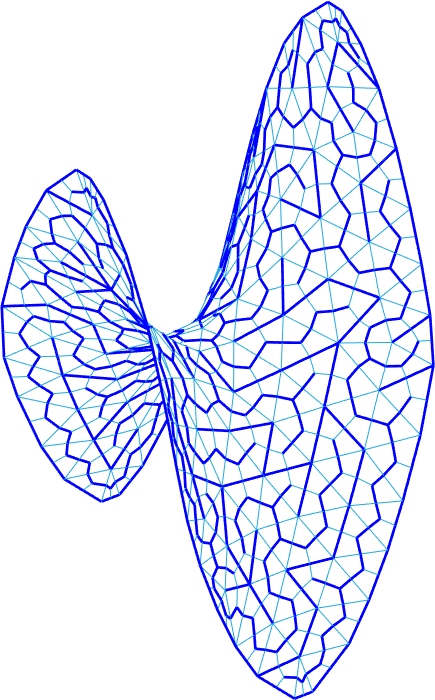
\includegraphics[height=0.17\textwidth]{figures/saddle/ours/006_nuc_st_view}
%}
%\subfloat[Top View]{
%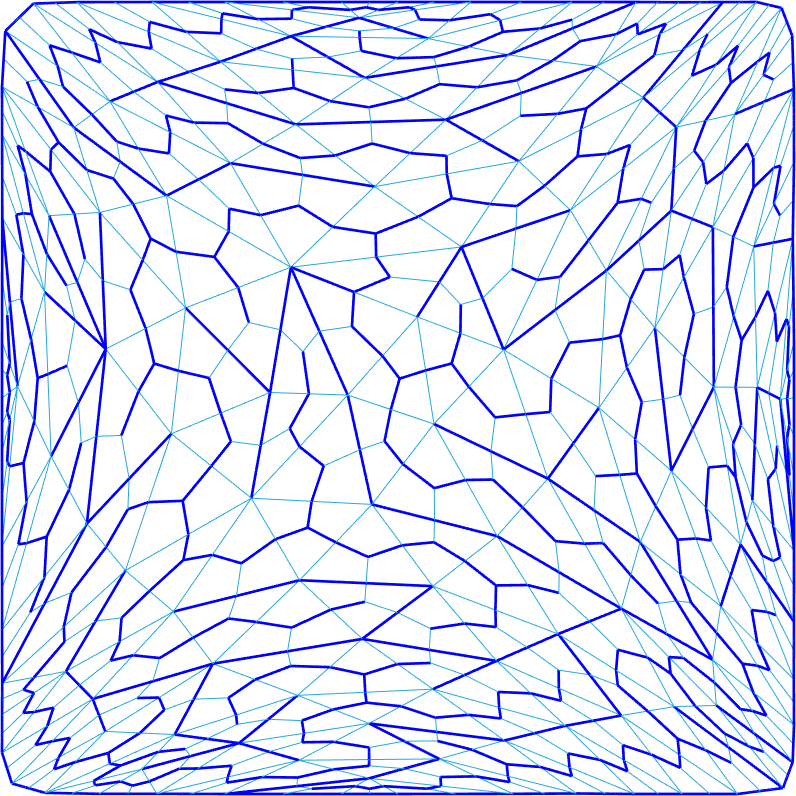
\includegraphics[height=0.17\textwidth]{figures/saddle/ours/006_nuc_top_view}
%}
%\subfloat[Coverage]{
%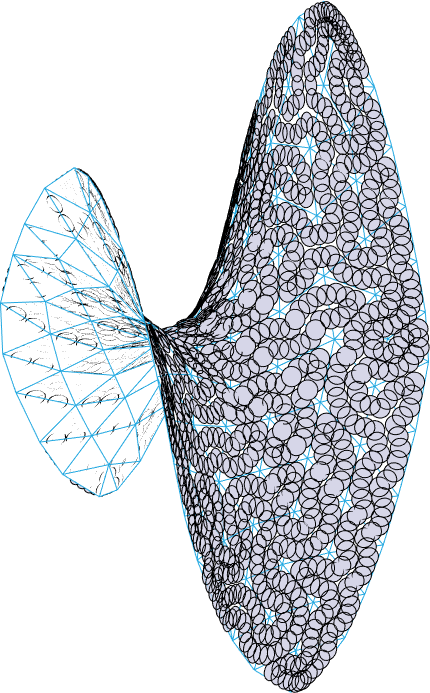
\includegraphics[height=0.17\textwidth]{figures/saddle/ours/006_tool_st_view}
%}
%
%\subfloat[NUC]{
%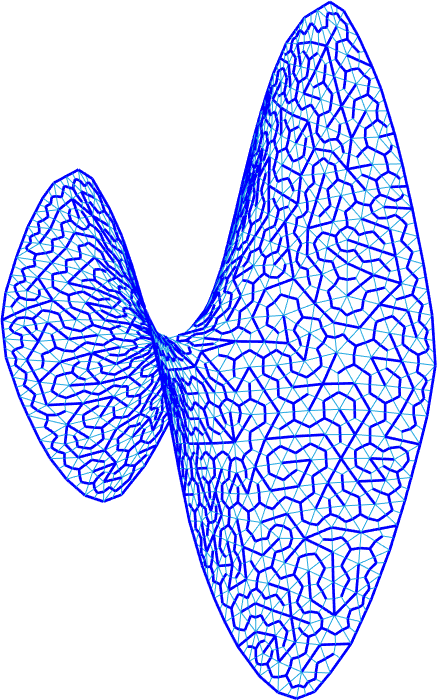
\includegraphics[height=0.17\textwidth]{figures/saddle/ours/003_nuc_st_view}
%}
%\subfloat[Top View]{
%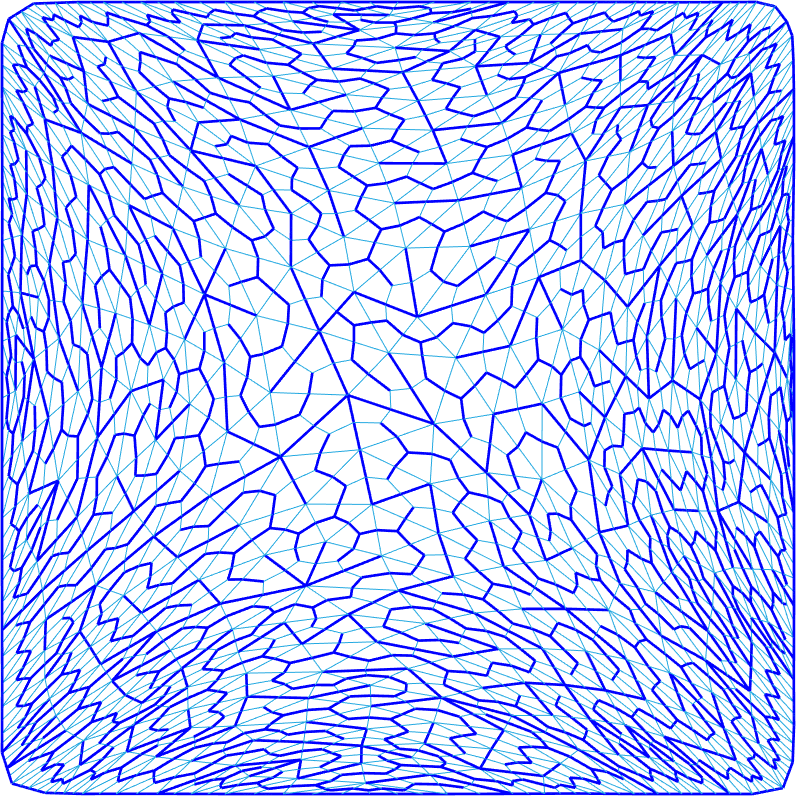
\includegraphics[height=0.17\textwidth]{figures/saddle/ours/003_nuc_top_view}
%}
%\subfloat[Coverage]{
%\includegraphics[height=0.17\textwidth]{figures/saddle/ours/003_tool_st_view}
%}
%
%\subfloat[NUC]{
%\includegraphics[height=0.17\textwidth]{figures/saddle/ours/0015_nuc_st_view}
%}
%\subfloat[Top View]{
%\includegraphics[height=0.17\textwidth]{figures/saddle/ours/0015_nuc_top_view}
%}
%\subfloat[Coverage]{
%\includegraphics[height=0.17\textwidth]{figures/saddle/ours/0015_tool_st_view}
%}
\subfloat[NUC]{
\includegraphics[height=0.17\textwidth]{figures/new_saddle/ours/sparse_nuc}
}
\subfloat[Top View]{
\includegraphics[height=0.17\textwidth]{figures/new_saddle/ours/sparse_nuc_top}
}
\subfloat[Coverage]{
\includegraphics[height=0.17\textwidth]{figures/new_saddle/ours/sparse_nuc_tool}
}

\subfloat[NUC]{
\includegraphics[height=0.17\textwidth]{figures/new_saddle/ours/middle_nuc}
}
\subfloat[Top View]{
\includegraphics[height=0.17\textwidth]{figures/new_saddle/ours/middle_nuc_top}
}
\subfloat[Coverage]{
\includegraphics[height=0.17\textwidth]{figures/new_saddle/ours/middle_nuc_tool}
}

\subfloat[NUC]{
\includegraphics[height=0.17\textwidth]{figures/new_saddle/ours/dense_nuc}
}
\subfloat[Top View]{
\includegraphics[height=0.17\textwidth]{figures/new_saddle/ours/dense_nuc_top}
}
\subfloat[Coverage]{
\includegraphics[height=0.17\textwidth]{figures/new_saddle/ours/dense_nuc_tool}
}
\caption{The coverage path of surface sub-facets generated by the proposed algorithm. The top-view of the resulting paths are illustrated, 
and simulated coverage results by a circular tool of different size are shown:  
(a)(b)(c) 1.21mm, (d)(e)(f) 0.57mm, and (g)(h)(i) 0.27mm.  }\label{fig:saddle_ours}
\end{figure}



% <T> We state this at the beginning of this section, in case that the reviewer cannot find a "formal proof" of the claimed contribution. 
%\textbf{Surface Homeomorphism. }
%The proposed algorithm does not have any constraint on the topological connectedness (simply/multiply-connectedness) of the target region. 


\begin{table}[t]
\centering
\caption{Performance of Various Coverage Paths on Saddle Surface}\label{tab:coverage_rate}
\begin{tabular}{c|c|c}
\hline
Methods & Tool Radius ($r$) & Coverage Rate \%\\
\hline
\hline
Boust. Horizontal & \multirow{4}{*}{1.21mm} & 63.46\%\\
\cline{1-1}\cline{3-3}
Boust. Vertical & &63.46\%\\
\cline{1-1}\cline{3-3}
Spiral & &51.80\%\\
\cline{1-1}\cline{3-3}
Ours & & \textbf{87.25\%}\\
\hline
Boust. Horizontal & \multirow{4}{*}{0.57mm} & 69.38\%\\
\cline{1-1}\cline{3-3}
Boust. Vertical & &69.38\%\\
\cline{1-1}\cline{3-3}
Spiral & & 54.85\%\\
\cline{1-1}\cline{3-3}
Ours & & \textbf{91.01\%}\\
\hline
Boust. Horizontal & \multirow{4}{*}{0.27mm} & 72.37\%\\
\cline{1-1}\cline{3-3}
Boust. Vertical & & 72.37\%\\
\cline{1-1}\cline{3-3}
Spiral & & 56.34\%\\
\cline{1-1}\cline{3-3}
Ours & & \textbf{92.45\%}\\
\hline
\end{tabular}
\end{table}


\section{Experiments}\label{section_experiment}
The proposed algorithm generates non-revisiting uniform coverage paths on any given mesh surface. 
In this section, simulated comparisons and real-world test cases are presented, emulating a coverage task performed 
on the object's surface by a non-particle contact tool. The effect of different tool sizes is studied, as well as 
comparisons with traditional coverage paths. 
The supplementary video with details of the simulations and the real-world coverage task can be found at: \\\url{https://youtu.be/eb2_LdGoKQA}


\begin{figure}[t]
\centering
\includegraphics[width=0.14\textwidth]{figures/bunny/bunny_001}
\includegraphics[width=0.14\textwidth]{figures/bunny/bunny_0005}
\includegraphics[width=0.14\textwidth]{figures/bunny/bunny_0003}
\caption{NUC path solutions generated on the Standford bunny mesh with resolution $r$ = 1.21mm (left), $r$ = 0.57mm (middle) and $r$ = 0.27mm (right). 
}\label{fig:bunny}
\end{figure}

\begin{figure}[t]
\centering
\includegraphics[width=0.22\textwidth]{figures/simu_illustration/turbine}
\includegraphics[width=0.22\textwidth]{figures/simu_illustration/gearbox}
\caption{NUC path solutions on a turbine (left) and a gearbox object (right).}\label{fig:exp_arbitrary}
\end{figure}



\begin{table}[t]
\centering
\caption{NUC Performance on Testing Objects}\label{tab:computation_time}
\begin{tabular}{c|c|c|c|c}
\hline
Object & Facets & Re-meshing$^1$ & Subdivision & NUC \\
\hline
\hline
%Bunny ($r=1.00mm$) & 1760 & 3.25s& 72.78ms& 57.00ms\\
Bunny (sparse) & 1760 & 3.25s& 72.78ms& 57.00ms\\
\hline
Bunny (middle) & 4934 & 3.23s& 277.20ms& 276.70ms\\
\hline
Bunny (dense) & 12475& 6.88s& 958.34ms& 1.21s\\
\hline
Turbine & 17977& 55.09s& 1.61s& 2.23s\\
\hline
Gearbox & 21301& 43.95s& 2.05s& 3.14s\\
\hline
\end{tabular}
\begin{tablenotes}
\item $^1$ Re-meshing step carried out prior in Meshlab~\cite{Cignoni2008Meshlab}.
\end{tablenotes}
\end{table}


\subsection{Comparisons on Saddle Surface}\label{section_exp_saddle}
The performance of the proposed algorithm is compared in detail with various coverage path planning algorithms by extensive testing on a classic non-planar object, a saddle surface. 
The top view of the saddle surface is a square (side length 34mm), thus re-meshing the surface into grids and projecting the template coverage paths are straightforward.
Given the contact size of the tool (say $r$=1.21mm case), the surface is first re-meshed with a resolution such that the central area of the saddle surface would not be over-covered.  
%(15 horizontal lines and 15 vertical lines, shown in Fig.~\ref{fig:exp_boust_horizontal}(a)) 
% TONG - pls check the above, I don't appreciate the re-meshing in the figures, and the vertical, horizontal and spiral paths in Figs 6, 7, 8, top left do not represent the re-meshing as far as I can see, but the classic template coverage path used, with the deformed tool coverage as the reference is the radius on the 3D saddle. I feel the above is not properly worded.
The coverage results with different tool sizes using existing algorithms are shown in Fig.~\ref{fig:exp_boust_horizontal}, Fig.~\ref{fig:exp_boust_vertical} and Fig.~\ref{fig:exp_spiral}. 
Although the paths are uniform in the projective square region, they are non-uniform on the saddle surface. 
In contrast, see Fig.~\ref{fig:saddle_ours} for the illustration of the proposed algorithm. 
Given the size of the tool contact point, the mesh is re-sampled, re-meshed, and refined into appropriate resolutions, and the NUC is generated by the proposed algorithm. 
The performance of different coverage motions can be measured by calculating the coverage rate, as shown in Table.~\ref{tab:coverage_rate}. 
Since no over-coverage appears, the covered area for all testings is calculated as the multiplication of the tool width ($2r$) and the length of the coverage path, and the coverage rate is the proportion of covered area in the whole mesh. 

\begin{figure*}[t]
\centering
\subfloat[Object Modelling]{
\includegraphics[width=0.22\textwidth]{figures/real_world/meshlab_model}
}
\subfloat[Re-meshing]{
\includegraphics[width=0.22\textwidth]{figures/real_world/remesh}
}
\subfloat[NUC Generation]{
\includegraphics[width=0.21\textwidth]{figures/real_world/simu}
}
\subfloat[Real-World Execution]{
\includegraphics[width=0.205\textwidth]{figures/real_world/demo_smaller}
}
\caption{Real-world implementation. 
(a) The surface of the object is firstly modelled into a mesh. 
(b) The surface mesh is repaired and re-sampled. The size of facets is appropriately chosen based on the tool size. 
(c) Taking the nonlinear manipulator kinematics into consideration, the coverable area on the surface has been visualised in a refined manner. 
A NUC solution is generated within the coverable area. 
(d) The real-world manipulator is tracking the NUC solution. 
}\label{fig:exp_real_world}
\end{figure*}

\subsection{Illustration on Arbitrary Object Surfaces}
In this subsection, the proposed algorithm is applied to arbitrary meshes. 
%We assume that a proper-size tool matching the mesh facet size is always obtainable to perform the coverage task. 
In Fig.~\ref{fig:bunny}, the NUC solutions on the Stanford bunny object are visualised. 
The proposed algorithm can generate the NUC solution on all meshes, while the physical uniformity depends on the distribution of mesh facet centers. 
In Fig.~\ref{fig:bunny} (left), the bunny was re-meshed by a sparse mesh resolution (corresponding to a large-size tool, 1.21mm) and the NUC solution is constructed. The bunny ears and feet are too winding to be modelled by the given mesh resolution, so the remeshing at these sub-regions have to be in a smaller facet size which leads to potential over-coverage. 
Most areas except ears and feet can be uniformly covered. 
See illustration in Fig.~\ref{fig:bunny} (middle), in a finer resolution (corresponding to a middle-size tool, 0.57mm), the feet can be appropriately modelled in the desired facet size, which indicates that the coverage of feet would be non-overlapping. 
Finally, in an extremely high resolution shown in Fig.~\ref{fig:bunny} (right), the facets are uniformly distributed on the ears, thus the physical uniformity of the coverage task on the bunny ears is established. 
In Fig.~\ref{fig:exp_arbitrary}, more testings are carried out on a turbine object and a gearbox object. 
The computational time for all testing cases are reported in Table.~\ref{tab:computation_time}. 
The reader is referred to the supplementary video for further illustrations. 


\subsection{Real World Experiments}
A real-world NUC task for manipulator tracking is illustrated to show the proposed algorithm in action on a real robot, as illustrated in Fig.~\ref{fig:exp_real_world}. 
A fixed-base UR5 manipulator is utilised, whereas the object to be inspected is an HRI robot HAIBAO~\cite{Xiong2011Haibao}. 
The surface is non-planar. The boundary of the coverable region is constrained in this example by the non-linear manipulator kinematics and collision checking. 
Singular manipulator configurations are disregarded, and the obstacles considered in the collision module are the HAIBAO body and the table. 
We modelled the surface into a mesh from 3D cloud data, which was then re-meshed to generate an unstructured mesh. 
%The resolution of the reconstructed mesh is carefully determined such that, after edge subdivision, the size of sub-facets aligns with the tooling size inf the manipulator end-effector. 
Since we do not impose any constraint on the topological layout of the mesh vertices, such remeshing can be easily attained. Meshlab~\cite{Cignoni2008Meshlab} was used for this step. 
The NUC solution on the surface was calculated in MATLAB with the code provided, identifying the desired manipulator task path. In this example, the smooth manipulator joint trajectory 
seen in the supplementary video was then generated by cubic interpolation and executed by the robot controller.

\section{Conclusion}\label{section_conclusion}
A novel construction for coverage planning of any given non-planar surface has been proposed in this work. 
The key problem that the work overcomes is the non-existence of a homeomorphic mapping from planar regions to non-planar surfaces that keeps 
the uniformity of path waypoints on the surface. The problem is fundamentally caused by the non-zero curvature which is prevalent everywhere on a non-planar surface, which cannot be addressed by cellular decomposition approaches 
from a global perspective. 

A uniform non-revisiting coverage path of the surface is equivalent to visiting a set of non-repeated, uniformly sampled waypoints that it is shown must be unstructurally laid on the surface.  
Then, this research considered the coverage path generation by letting a path 
be continuously deformed until exhaustively filling the target surface area. 
The existence of a NUC path on the edge-subdivided polygonal mesh of any arbitrarily 
shaped object surface was proven, and a practical algorithm was proposed to find a valid NUC resulting path. 
This makes the proposed scheme prominently applicable in coverage tasks under nonlinear manipulator constraints. 
The algorithm is compatible with any high-level cellular decomposition method, and admits any heuristics with the aim to improve the quality of the resulting path. 
Extensive illustrations and a real-world implementation on a manipulator coverage task have been presented to show the validity of the proposed algorithm, and the coverage improvements that can be achieved (up to 92.45\%) when compared with traditional coverage algorithms such as a homeomorphic Boustrophedon mapping (up to 72.37\%). 
These have been supplemented by a detailed video and an open sources implementation in MATLAB for the benefit of the research community. 

\bibliographystyle{ieeetr} %% setting the cite style
\bibliography{IEEEabrv,geometric_cpp}

\vfill

\end{document}


